\documentclass[12pt]{article}

\usepackage[french]{babel}
\usepackage[utf8]{inputenc}
\usepackage{amsmath,amssymb}
\usepackage{parskip}
\usepackage{graphicx}
\usepackage{multicol}
\usepackage{amsmath}
\usepackage{float}


% Margins
\usepackage[top=1.5cm, left=2cm, right=2cm, bottom=2.0cm]{geometry}
% Colour table cells
\usepackage[table]{xcolor}

% Get larger line spacing in table
\newcommand{\tablespace}{\\[1.25mm]}
\newcommand\Tstrut{\rule{0pt}{2.6ex}}         % = `top' strut
\newcommand\tstrut{\rule{0pt}{2.0ex}}         % = `top' strut
\newcommand\Bstrut{\rule[-0.9ex]{0pt}{0pt}}   % = `bottom' strut

%%%%%%%%%%%%%%%%%
%     Title     %
%%%%%%%%%%%%%%%%%
\title{Synthèse Télécommunication LELEC1930}
\author{Jacques HOGGE}
\date{\today}

\begin{document}
\maketitle
\newpage
\tableofcontents
\newpage

\section{Introduction}
Quelques définitions:

\textbf{Télécommunication} : Transmission d'information sous la forme de signaux électriques sur un canal de communication.

\textbf{Signal} : Évolution de la tension en fonction du temps.

	\subsection{Canaux de communication}
		2 type de canaux:
		\begin{itemize}
			\item \textbf{Filaire} : Ligne téléphonique, câbles coaxiaux, fibre optique, \dots
			\item \textbf{Sans fils} : Onde électromagnétique dans l'air ou espace.
		\end{itemize}
		
		3 éléments les caractérisent :
		\begin{itemize}
			\item \textbf{Atténuation} : Diminution de l'amplitude ou de la puissance d'un signal lors de sa transmission. Il augmente avec la distance
			\item \textbf{Bruit/Interférence} : Partie du signal ou on ne peut pas tirer de l'information.
			\item  \textbf{Distorsion/Dispersion} : Ensemble des modifications indésirable d'un signal. Il existe plusieurs source
			\begin{itemize}
				\item \textbf{Multitrajet} : Soit le signal arrive directement à la source, soit il rebondit sur des obstacles, le signal est alors découpé en plusieurs morceaux de moindre intensité mais répartis sur le temps.
				\item \textbf{Effet Doppler} : La fréquence des signaux qui s'approchent de nous est différente de ceux qui s'éloignent de nous.
			\end{itemize}
			
			\begin{figure}[H]
				\centering
				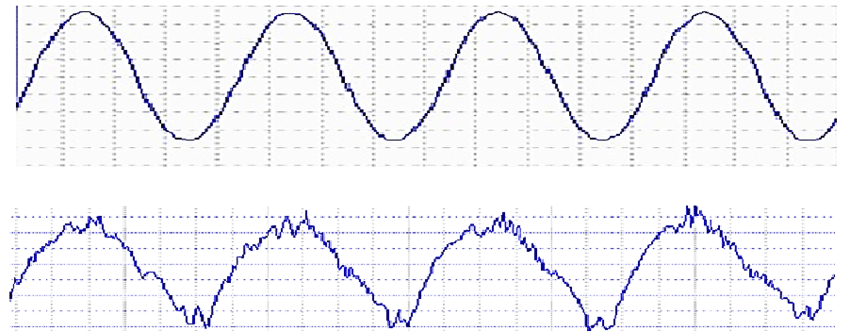
\includegraphics[width=\textwidth]{img/Distortion.png}
			\end{figure}
		\end{itemize}
	
	
	L'information est représentée sous la forme d'un signal. Cela veut dire que changer l'amplitude du signal ne change pas l'information. Mais la distorsion elle change l'information car le signal change de forme et donc modification du signal et de l'information.
	
\subsubsection*{3 moyens de représenter le signal :}
	\begin{itemize}
		\item \textbf{Signaux analogiques}
		\item \textbf{Signaux numériques}
		\item \textbf{Numérisation} : Transformation de signaux analogique en numérique.
	\end{itemize}
		\begin{figure}[H]
			\centering
			\includegraphics[width=0.6\textwidth]{img/Analogique-Numérique.png}
		\end{figure}
		
	\subsection{Transformation de Fourier}
		Moyen de représenter un signal par un ensemble de fréquence. Elle permet d'analyser un signal en une somme de sinusoïde = \textbf{Contenu fréquentiel}.
		\begin{figure}[H]
			\centering
			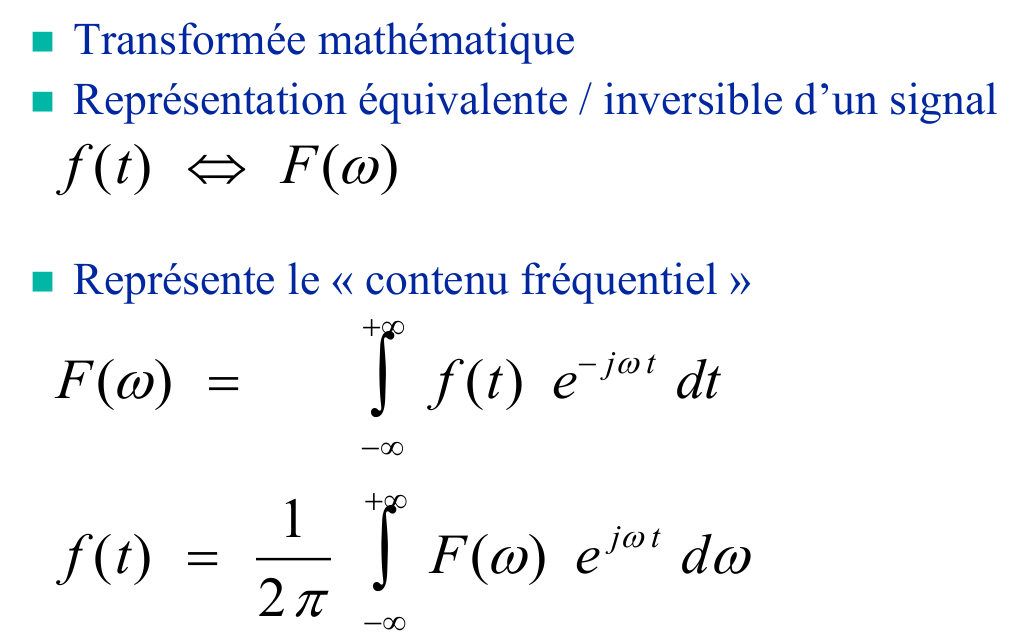
\includegraphics[width=0.6\textwidth]{img/Fourrier.png}
			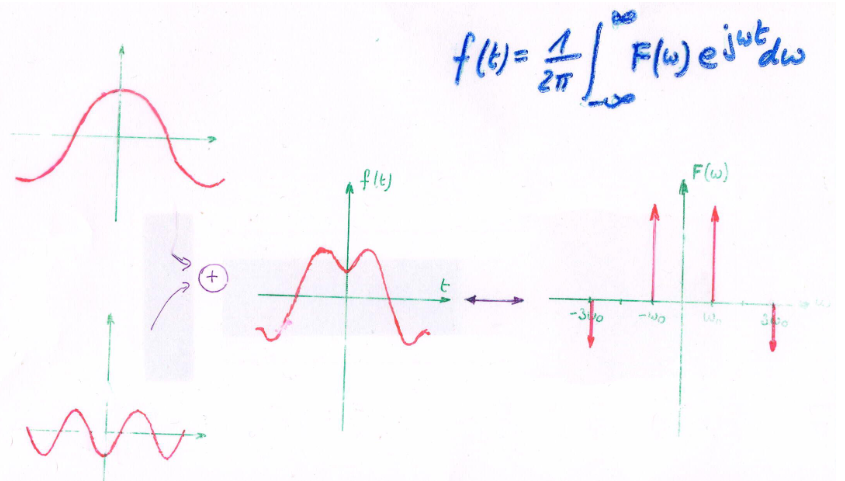
\includegraphics[width=0.6\textwidth]{img/FourrierExemple.png}
		\end{figure}
		
		On peut voir sur les schémas que la fonction $f(t)$ est la somme des 2 sinusoïdes dans l'exemple donné. Mais la fonction $F(\omega)$, si on ne regarde que du coté positif, $F(\omega)$ représente qu'il y a une sinusoïde à 10kHz (première flèche vers le haut) et un sinusoïde à 30kHz, celle-ci pointe vers le bas car elle commence à un nombre négatif sur le schéma.
		
	\subsection{Bande de Fréquence}
		Tous les systèmes de télécom sont limités en fréquence = la bande de fréquence du système.
		
		La \textbf{Modulation} permet de transposer un signal autour d'un fréquence définie, c'est utilisé pour partager les différentes bandes de fréquence.
		
		Un signal \textbf{modulé} est un signal \textbf{modulant} mis sur une \textbf{porteuse} à la fréquence désirée.
		
		Le \textbf{Multiplexage} permet de faire passer plusieurs informations sur un seul support de fréquence. Les différents symboles sont combinés grâce à un multiplexeur. Deux types:
		\begin{itemize}
			\item \textbf{Temporel}
			\item \textbf{Fréquentiel}
		\end{itemize}
		\begin{figure}[H]
			\centering
			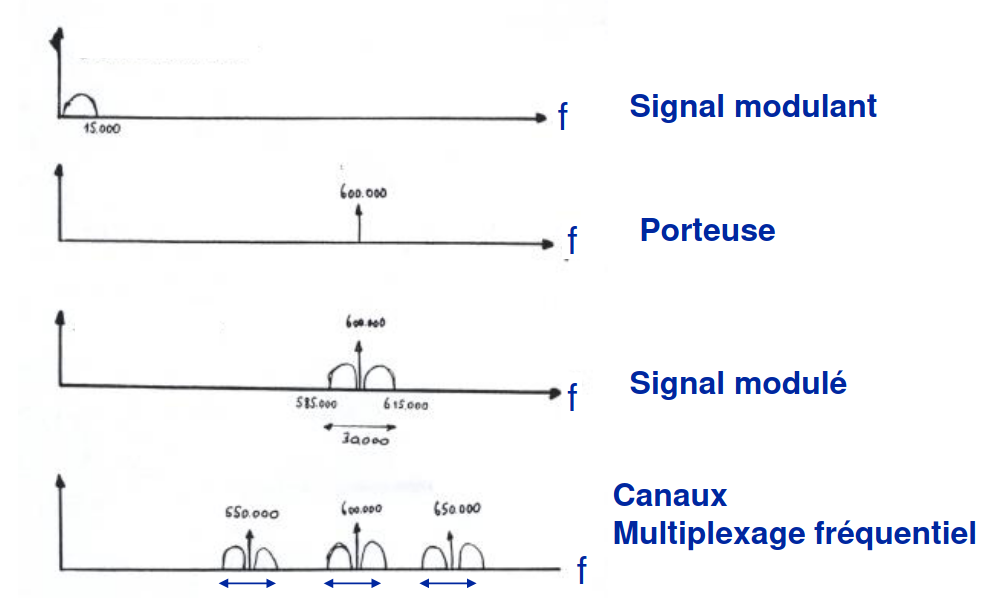
\includegraphics[width=0.6\textwidth]{img/Multiplexage.png}
		\end{figure}
	\subsection{Exemples}
		\subsubsection{Son}
			Un micro capture les ondes de pressions dûes à la voix sous la forme d'un signal électrique.
			
			Le haut-parleur lui reçoit le signal électrique et fait vibrer une membrane pour recréer le son.
			
			
		\subsubsection{Stéréo}
		
			Les sons gauches (G) et droites (D) sont envoyés ensemble sous un signal $S_1 = G+D$ donc la somme des 2. Grâce à ça les radios Mono peuvent recevoir le signal aussi. Un autre signal est aussi envoyé par la stéréo : $S_2 = G-D$. Le signal stéréo peut alors être recréé avec l'opération suivante


			\begin{align*} 
				G &=  S_1 + S2 = (G+D) + (G-D) = 2G \\ 		
				D &=  S_1 - S2 = (G+D) - (G-D) = 2D
			\end{align*}
			
			On va avoir un effet de compression car $S_2$ est souvent très petit par rapport à $S_1$. $S_2$ a un contenu fréquentiel faible et aura donc une bande de fréquence plus faible.
		
		\subsubsection{TV analogique}
		
			On joue sur la luminance (niveau de gris) des lignes est envoyée par pulsation de synchronisation (Synchronizing pulse) entre chaque ligne.

			Un canon à électrons envoie la lumière ligne après ligne sur l'écran pour afficher une image
			
\begin{figure}[H]
\centering
\begin{minipage}{.5\textwidth}
  \centering
  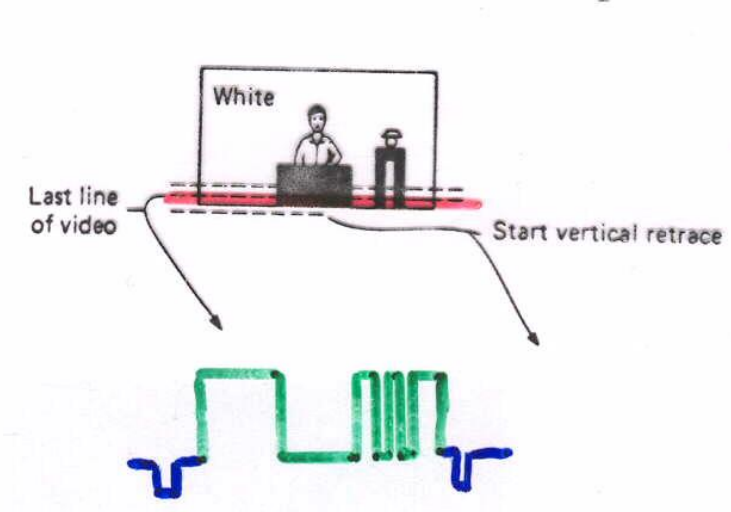
\includegraphics[width=.5\textwidth]{img/TV1.png}
\end{minipage}%
\begin{minipage}{.5\textwidth}
  \centering
  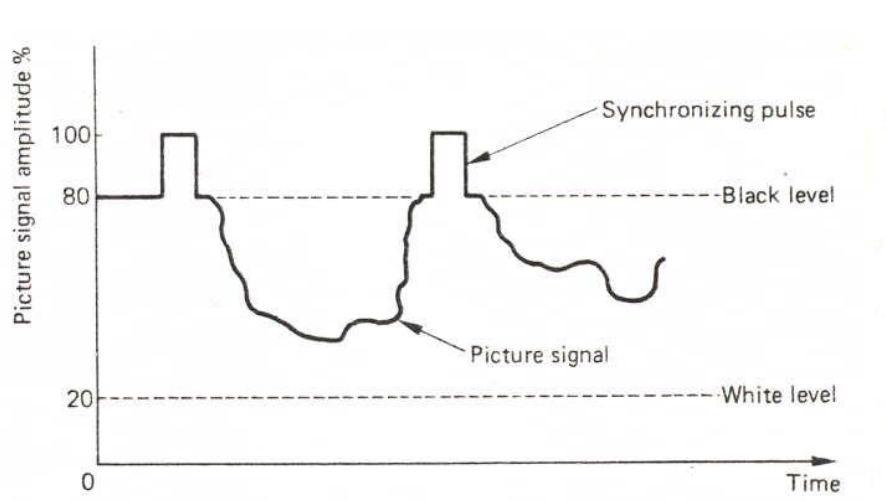
\includegraphics[width=.5\textwidth]{img/TV2.png}
\end{minipage}
\end{figure}
			
			Pour les couleurs, on fait pareil que la stéréo, on garde l'envoi de luminance pour que les vieilles TVs fonctionnent encore.
			
			On a donc \textit{RGB} (red,green,blue) et \textit{YUV} les signaux (luminance Y et chrominance U V)
			
			\begin{align*} 
				Y &= 0.3\textcolor{red}{R} + 0.59\textcolor{green}{G} + 0.11\textcolor{blue}{B}\\
				U &= 0.493(\textcolor{blue}{B}-Y)\\
				V &= 0.877(\textcolor{red}{R}-Y)
			\end{align*}
	\subsection{Signaux numérique}
		C'est simple, c'est du binaire.
		
		Si on a un signal analogique et que on veut en faire un numérique $\rightarrow$ Numérisation.
		
		Il peut y avoir des erreurs dans ce que on a transmis et ce que on lit.
		
	\subsection{Numérisation}
		Passer d'un signal analogique à un signal numérique. On va devoir \textbf{Échantillonner} le signal (captures de valeur à intervalles fixes). Car le signal numérique a des avantages :
		\begin{itemize}
			\item Traitement et stockage de l'information.
			\item Regénération du signal par des codes correcteurs et détecteurs d'erreur.
		\end{itemize}
		
		Signal analogique représenté par des valeurs continues ($\mathbb{R}$) et signal numérique par des valeurs discrètes (0 ou 1).
		
		Le procédé de transformation est appelé \textbf{Quantification}, on remplace les valeurs continues reçues par les valeurs discrètes qui s'en rapprochent le plus.
		
		Avantage du numérique est que le bruit dans l'analogique sera filtré s'il est faible.
		
		Lors de l'échantillonnage, il ne faut pas prendre une fréquence trop grande sous peine d'avoir beaucoup d'erreur. Le \textbf{Théorème de Shannon} certifie que il n'y a aucune perte si la fréquence d'échantillonnage est au moins 2 fois supérieure à la fréquence maximum du signal.
		
		\begin{figure}[H]
			\centering
			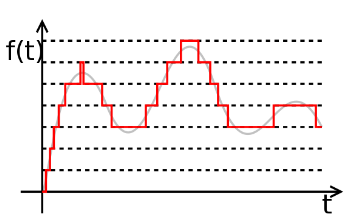
\includegraphics[width=0.6\textwidth]{img/Quantification.png}
		\end{figure}		
		
		
		

\newpage

\section{Lignes}
		
	Il existe plusieurs types de lignes:
	\begin{itemize}
		\item unifilaire
		\item bifilaire
		\item coaxiale
		\item fibre optique
		\item à ruban
		\item \dots
	\end{itemize}
		
		Elles dépendes de leur géométrie, des matériaux et des conditions, \dots
		
	\subsection{Modélisation d'une ligne}
	
		Une ligne est représentée comme  une résistance $R'$ ($\Omega/m$), une conductance $G'$, une inductance $L'$ et une capacité $C'$. Le morceau représenté si dessous se répète tous le long de la ligne.
		
		\begin{figure}[H]
			\centering
			\includegraphics[width=0.6\textwidth]{img/ModélisationLigne.png}
		\end{figure}		
		
		\begin{itemize}
			\item \textbf{$R'$} : Résistance du matériau (cuivre) qui transmet le signal $\rightarrow$ atténuation.
			\item \textbf{$L'$} : Inductance champ magnétique produit par un fil et qui impacte l'autre.
			\item \textbf{$C'$} : Effet de capacité entre les 2 fils.
			\item \textbf{$G'$} : Conductance, très grande résistance entre les 2 fils (air ou isolant) mais courant peut tout de même parfois passer légèrement à travers.
		\end{itemize}
		
		Ces paramètres varient suivant le type de ligne, la fréquence ou le matériel utilisé.
		
		L'équations des télégraphistes nous donnent la relation suivante :
		\begin{equation}
			\cfrac{\delta^2v}{\delta z^2} = LC\cfrac{\delta^2 v}{\delta t^2} + (RC + LG)\cfrac{\delta v}{\delta t} + RGv
		\end{equation}
		
		Si les pertes sont négligeables \textit{(R = G = 0)} :
		\begin{equation}
			\cfrac{\delta^2 v}{\delta z^2} = LC\cfrac{\delta^2 v}{\delta t^2}
		\end{equation}
		
		Elle fait le lien entre la variation de la tension en fonction de la position et un variation de la tension en fonction du temps.
		
		
	\subsection{Effet pelliculaire}
		Effet électromagnétique qui repousse les lignes de courant  vers la surface du conducteur. Les électrons vont s'amasser sur les bords.
		Diminue la surface de la ligne qui est effectivement parcourue par du courant et donc augmente la resistance de celui-ci comme $\sqrt{f}$, il est causé par la création d'un champ magnétique.
		
		\begin{align*}
			\nearrow \text{fréquence} \Rightarrow \nearrow \text{effet péliculaire} \Rightarrow \nearrow \text{résistance} \Rightarrow \nearrow \text{pertes}
		\end{align*}
			
	\subsection{Atténuation}
		Peut être calculé comme $10\log(P_{1}/P_{2})$, avec $P_1$ la puissance d'entrée et $P_2$ la puissance de sortie. Cette atténuation se calcule en dB(décibels).
		
		On sait que $P = \cfrac{V^2}{R}$, donc $\cfrac{P_1}{P_2} = \cfrac{v_{1}^{2}}{v_{2}^{2}}$
		
		\begin{equation}
			10\log(P_{1}/P_{2}) = 10\log(\cfrac{v_{1}^{2}}{v_{2}^{2}}) = 20\log(\cfrac{v_{1}}{v_{2}})
		\end{equation}
		
	\subsection{Dispersion}
		La \textbf{Dispersion} est une sorte de distorsion du signal et donc qui impacte l'information.
		
		Soit le nombre de pulsion $\omega = 2 \pi f$, le vecteur d'onde $\beta = \cfrac{2\pi}{\lambda}$, et $\lambda$ la longueur d'onde, on a la vitesse de phase (vitesse de propagation).
		\begin{equation}
			v_{ph} = \cfrac{\omega}{\beta}
		\end{equation}
		
		La dispersion d'un signal vient des différentes vitesses de déplacement des fréquences constituant une onde. L'onde a tendance à s'étaler sur le temps plus la ligne est longue.
		
	\subsection{Impédance caractéristique}
		Permet de connaitre le rapport de tension/courant utile dans beaucoup de systèmes pour savoir quelle tension on va récupérer en envoyant un certain courant. \textbf{Impédance caractéristique} désigne l'impédance en supposant que la ligne est infinie.
		
		La loi de Ohm caractérise une tension $v$ en fonction d'un résistance $r$ (ou $z$ pour résistances avec des nombres complexes) et d'un courant $i$.
		\begin{equation}
			v = ri\  \text{ou} \  v = zi
		\end{equation}
		
		$z$ est totalement réel pour une résistance pure et totalement imaginaire pour une inductance/capacité pure.
		
		Dans le cas d'une ligne infinie, l'impédance d'entrée est égal à l'impédance caractéristique de la ligne $Z_{in} = Z_c$\footnote{Voir slide 26 chap 2}.
		
	\subsection{Exposant de propagation}
		Il arrive que il y ait de la dispersion (déphasage) et de l'affaiblissement linéique (atténuation). Soit $\alpha$ l'atténuation et $\beta$ le déphasage, on peut calculer l'exposant de propagation $\gamma$:
		\begin{equation}
			\gamma = \sqrt{(R + j \omega L)(G + j \omega C)} = \alpha + j \beta
		\end{equation}
		
		Normalement, dans une ligne, $G$ est négligeable. Deux cas se présentent :
		
		\subsubsection{Cas 1}
			Dans le cas où, $\omega L << R$, correspond au cas où le fil a beaucoup de résistance.
			
			L'exposant de propagation en considérant $G$ et $\omega L$ nuls (car ils sont négligable au vu des hypothèses de ce cas) devient :
			
			\begin{figure}[H]
				\centering
				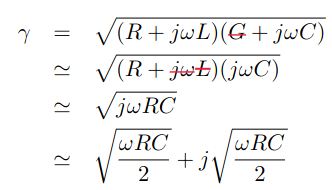
\includegraphics[width=0.4\textwidth]{img/1.png}
			\end{figure}	
			
			L'impédance caractéristique en considérant $G$ et $\omega L$ nul devient :
			
			\begin{figure}[H]
				\centering
				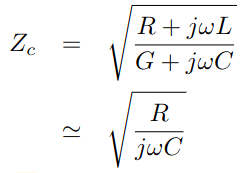
\includegraphics[width=0.3\textwidth]{img/2.png}
			\end{figure}	
				
		\subsubsection{Cas 2}
			Dans le cas où, $\omega L >> R$, correspond au cas où le fil a peu de résistance.
			C'est une bonne situation car il y a peu de distortion.
			
			L'exposant de propagation en considérant $G$ nul (car il est négligable) devient :
			
			\begin{figure}[H]
				\centering
				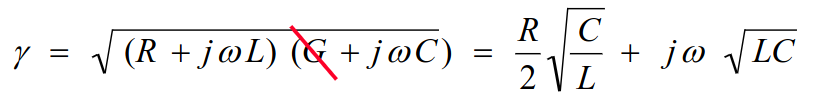
\includegraphics[width=0.6\textwidth]{img/3.png}
			\end{figure}	
			
			L'impédance caractéristique en annulant $G$ et $R$.
			
			\begin{figure}[H]
				\centering
				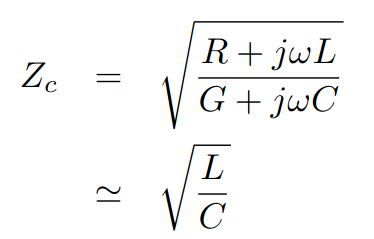
\includegraphics[width=0.2\textwidth]{img/4.png}
			\end{figure}	
			
			$\alpha$ est indépendant de $\omega$ et $\beta$ proportionnel à $\omega$. À cela s'ajoute $Z_c$ qui est réel et indépendant de $\omega$.
			
						
	\subsection{Pupinisation}
	
		Le cas des anciennes lignes téléphonique basse fréquences. Plus utilisé maintenant avec ADSL/VDSL.
		
		Pour le cas d'une ligne téléphonique $\omega L << R$, on va faire une pupinisation. C'est le fait d'insérer des inductances le long de la ligne pour augmenter artificiellement L. Avec ça, on a une réduction de l'atténuation le long de la ligne. On crée un filtre passe-bas.
		
		Mais cela n'est pas très bénéfique pour une certaine bande de fréquences car elle cause l'atténuation des fréquences supérieures. Vu qu'on a besoin de ces basses fréquences, on utilise plus cette technique \footnote{Voir graph Slides 34-35 chap 2}.
		
	\subsection{Lignes Bifilaire}
	
		Lignes constituée de fils parallèles séparés par un isolant, souvent rassemblé dans des quartes torsadées (quatre fils ensembles) ou encore dans une bottes de quartes (50 fils).
		
		On peut trouver de la Diaphonie (\textit{Bruit} / \textit{Crosstalk}). L'interférence d'un premier signal avec un autre (on peut par exemple entendre une autre conversation) qui passe dans un fil différent.
		
		Avantage :
		\begin{itemize}
			\item Faible coût
			\item Connexion facile
			\item Pré-installation dans les bâtiments
		\end{itemize}
		
		Déavantage :
		\begin{itemize}
			\item Faible atténuation aux basses fréquences
			\item Rayonnement important (problème de confidentialité, sensibilité aux interférences)
		\end{itemize}

\begin{figure}[H]
\centering
\begin{minipage}{.5\textwidth}
  \centering
  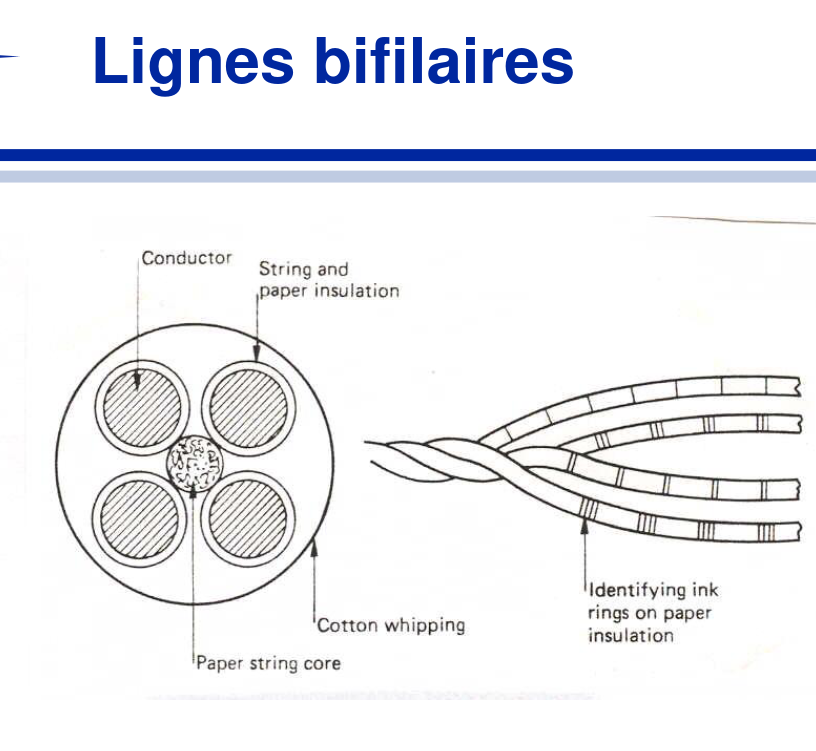
\includegraphics[width=.5\textwidth]{img/bifillaire.png}
\end{minipage}%
\begin{minipage}{.5\textwidth}
  \centering
  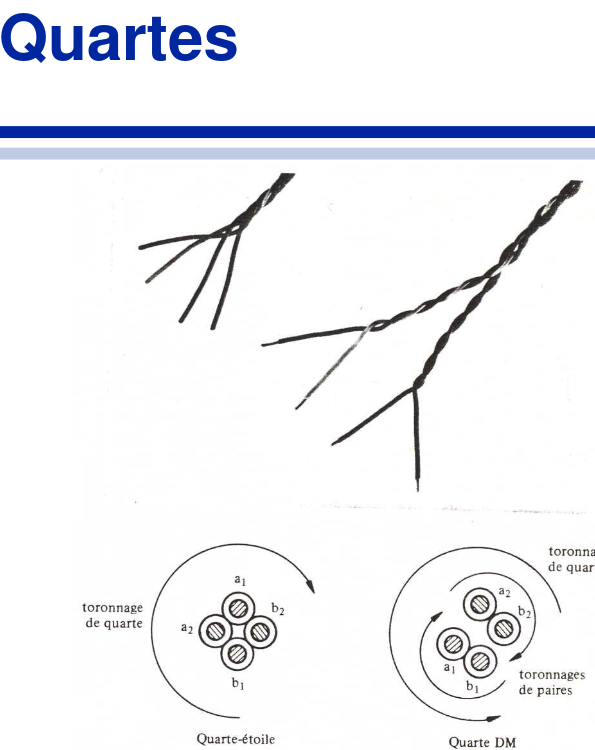
\includegraphics[width=.5\textwidth]{img/bifillaire2.png}
\end{minipage}
\begin{minipage}{.5\textwidth}
  \centering
  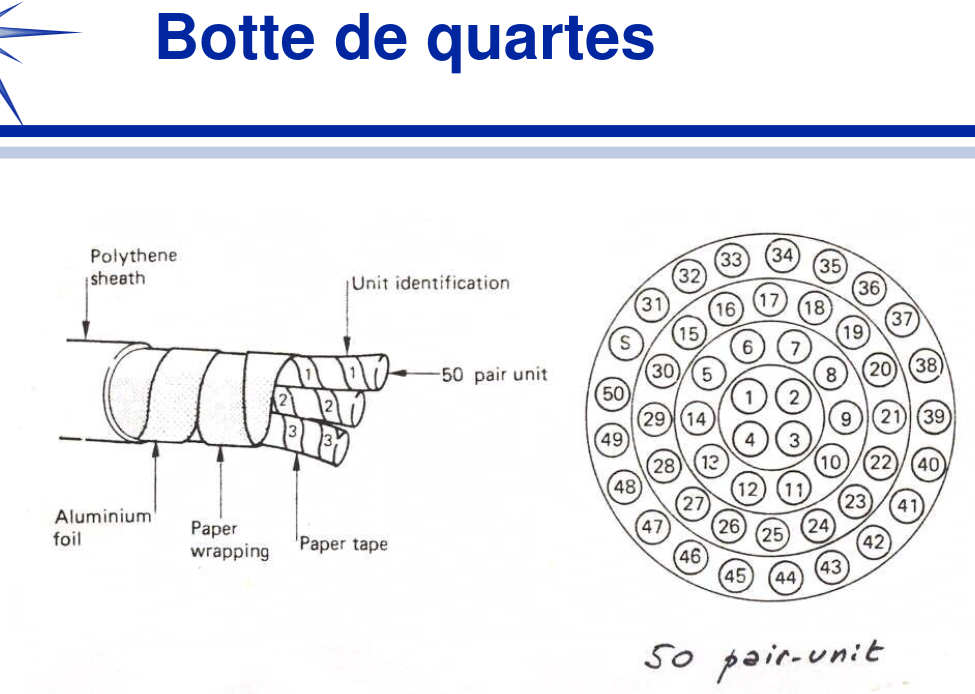
\includegraphics[width=.7\textwidth]{img/bifillaire3.png}
\end{minipage}

\end{figure}		
		
	\subsection{Cable coaxial}
		Câble composé d'une partie centrale (fil de cuivre) enveloppée d'un isolant, puis d'un blindage métallique tressée et enfin d'une gaine extérieure. Ce câble est utilisé pour la transmission de la télédistribution.
		
		Avantages :
		\begin{itemize}
			\item Large bande passante (\sim 500 MHz)
			\item Protection contre les interférences
			\item Technique éprouvée et répandue
			\item Facilité de réparation et de connexion
		\end{itemize}
		
		Désavantages :
		\begin{itemize}
			\item Fréquence limitée (\sim 500 MHz)
			\item Blindage jamais parfait
		\end{itemize}
		
		\begin{figure}[H]
\centering
\begin{minipage}{.5\textwidth}
  \centering
  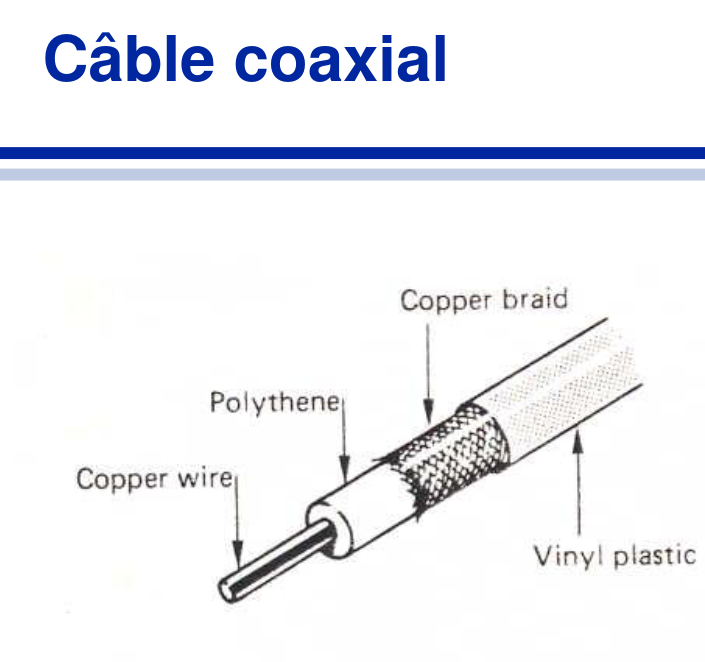
\includegraphics[width=.6\textwidth]{img/coaxial1.png}
\end{minipage}%
\begin{minipage}{.5\textwidth}
  \centering
  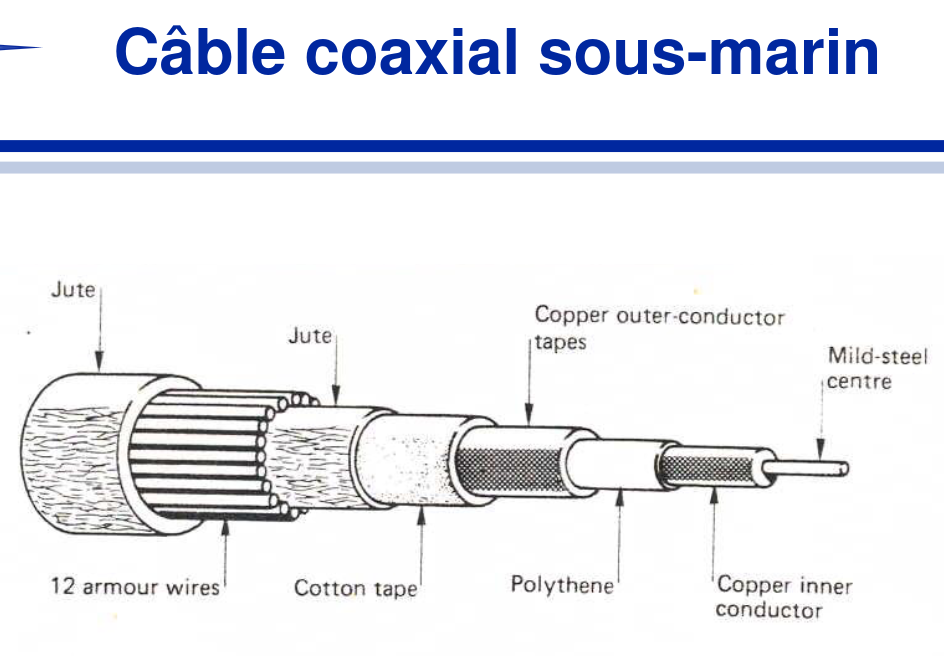
\includegraphics[width=.6\textwidth]{img/coaxial2.png}
\end{minipage}
\begin{minipage}{.5\textwidth}
  \centering
\end{minipage}

\end{figure}		

	\subsection{Fibre optique}
		C'est un conducteur de lumière en fil en verre ou plastique très fin qui transmet les données sous forme de lumière.
		
		Un \textbf{Mode} est un chemin emprunté par la lumiere par rapport à sa réflexion et réfraction dans la fibre optique.
		
		La \textbf{Dispertion intermodale} c'est un phénomène correspondant à l'existence de différentes vitesses possible pour la propagation des ondes. La distance parcourue par certains modes est différente de celle d'autre mode, il y a donc une dispersion du signal.
		
		Il y a plusieurs moyens d'envoyer un signal lumineux :
		\begin{itemize}
			\item Diode LED
			\item Diode Laser
			\item Diode Infrarouge
		\end{itemize}

		\textbf{Avantages :}
		\begin{itemize}
			\item Énorme bande passante
			\item Très faible attenuation
			\item Immunité à l'égard des rayonnement
			\item Isolation électrique
			\item Léger, fin, pas cher
		\end{itemize}
		
		\textbf{Désavantages :}
		\begin{itemize}
			\item Connexions difficiles
			\item Réparations difficiles
			\item Toujours en développement
		\end{itemize}
		
		\subsubsection{Manières de gérer les modes}
			\begin{enumerate}
				 \item \textbf{Fibre multimode à saut d'indice} : Les rayons réfléchissent plusieurs fois sur les parois avec un multitude d'angles différents. Le saut d'indice engendre des angles très fluctuants, il y a donc de la dispertion intermodale.
				 \begin{figure}[H]
				 	\centering
				 	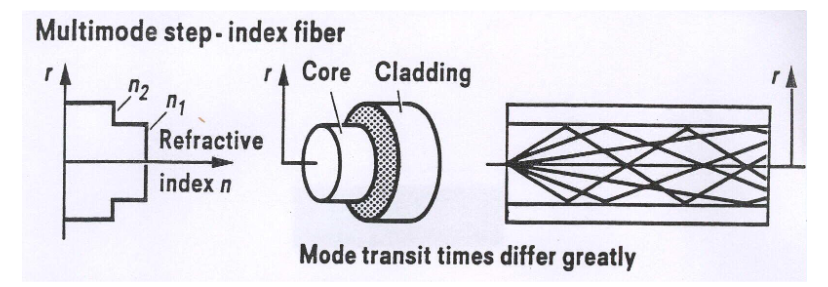
\includegraphics[width=\textwidth]{img/multimode.png}
				 \end{figure}
				 
				 \item \textbf{Fibre multimode à gradient d'indice} : On fait varier l'indice de réfraction plus l'on s'apporchera des parois afin que les différents faisceaux lumineux convergent vers le centre de la fibre. La dispersion intermodale est réduite.
				 
				 \begin{figure}[H]
				 	\centering
				 	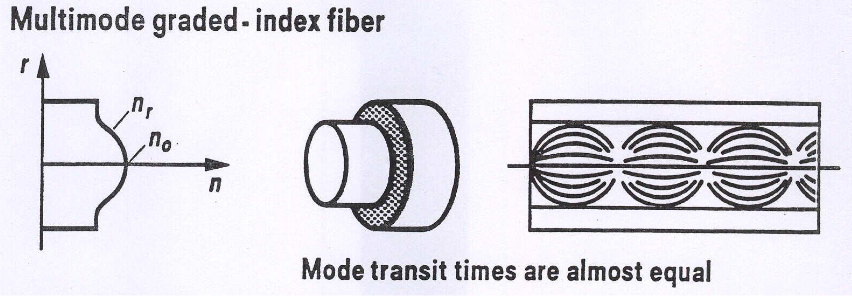
\includegraphics[width=\textwidth]{img/multimode2.png}
				 \end{figure}
				 
				 \item \textbf{Fibre Monomode} : un seul chemin au centre de la fibre. Une seule vitesse dans la fibre donc pas de dispertion intermodale.
				 
				 \begin{figure}[H]
				 	\centering
				 	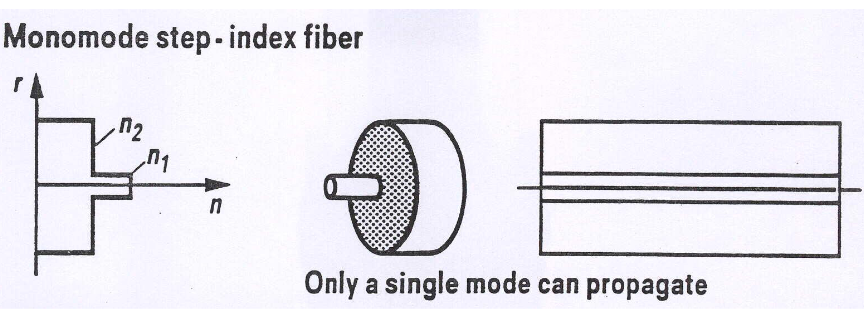
\includegraphics[width=\textwidth]{img/multimode3.png}
				 \end{figure}
			\end{enumerate}
			
			\subsubsection{Transmission dans une fibre optique}
				Un rayon rentre dans la fibre optique et est réfléchi à l'intérieur si celui-ci possède un angle adéquat qui est donc dans la range du cône d'appartenance et va parcourir la fibre optique en zigzag.
				

\newpage

\section{Propagation atmosphérique et Antennes}
	Les ondes intérragisse avec leur environnement, cela dépend de la fréquence, taille de l'objet rencontré, surface, matériaux, \dots
	
	il existe différente maniere de propagé les ondes:
	\begin{itemize}
		\item onde satellite
		\item onde ionosphère
		\item onde direct
		\item onde de sol
	\end{itemize}
	
	
	\subsection{Ondes direct}
		les ondes sont envoyé en ligne droite a une autre antennes. La porté est limité par l'horizon. Il y a aussi des interférence (distortion/dispersion) avec les onde réfléchie sur le sol.
		
		\begin{figure}[htp]
			\centering
			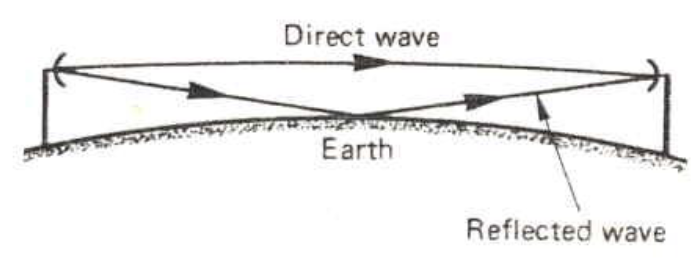
\includegraphics[width=0.7\textwidth]{img/onde_direct.png}
		\end{figure}
	
	\subsection{Ondes de sol}
		Ondes basse fréquences qui se propage généralement le long du sol car le fronts des ondes basses fréquences se déplacement perpendiculairement au sol.
		\begin{center}
			\begin{tabular}{c|c}
			\hline
			Fréquency & Range(Km)\\
			\hline
			100 kHz & 200\\
			1 MHz & 60\\
			10 MHz & 6\\
			100 MHz & 1.5\\
			\hline
		
		\end{tabular}
		\end{center}
		
	\subsection{onde ionosphérique}
		Avec l'effet de l'ionisation de de l'air par les UV du soleil et crée un "mur" contre les ondes et les réfléchie.
		Il y a 4 couches précises de la plus proche a la plus éloignée, $D,E,F_1,F_2$. pendant la nuit il ne reste que une seule couche nommé $F$
		
		\begin{figure}[htp]
			\centering
			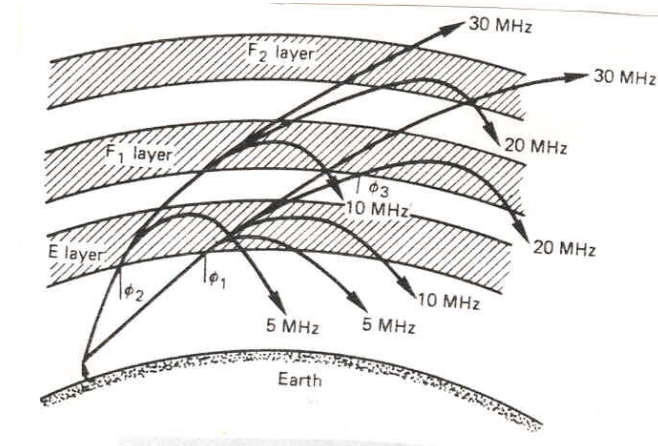
\includegraphics[width=0.7\textwidth]{img/refraction.png}
		\end{figure}
		
		Grace a cela, on peut propager les ondes entre continant. Fort utiliser pour les hondes haute fréquences.
		
		\textbf{MUF} est le Maximal Usable Frenquency, c'est la fréquence max que on est sure a 50\% que elle est réfléchie par la ionosphère.Elle est différente en fonction du jour ou de la nuit.
		
	\subsection{Onde par satellite}
		On a un satellite géostationnaire, qui reste au même endroit par rapport a la terre a qui on envoi le signal et qui le retransmet a d'autre antennes.
		
		\begin{figure}[htp]
			\centering
			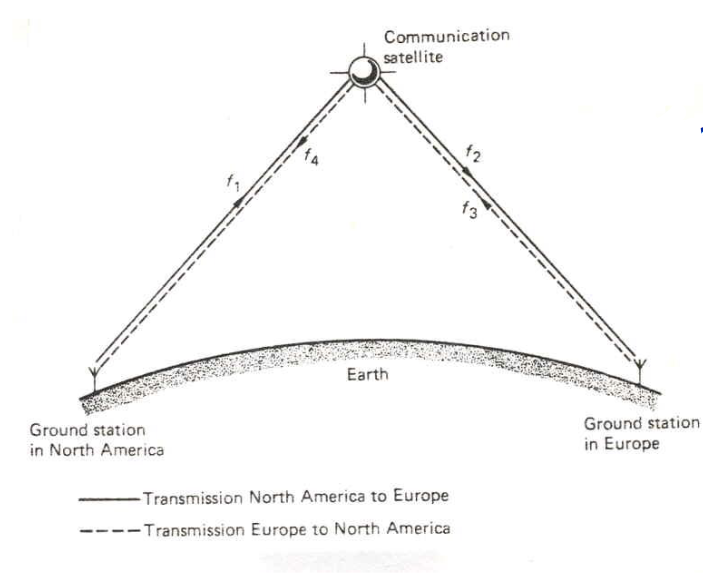
\includegraphics[width=0.7\textwidth]{img/satellite.png}
		\end{figure}
		
	\subsection{Antennes}
		C'est un dispositif qui peut émettre, ou recevoir des ondes électromagnétiques. Autour d'une antennes, on a a des champs magnétique et électrique.
	
		\begin{figure}[htp]
			\centering
			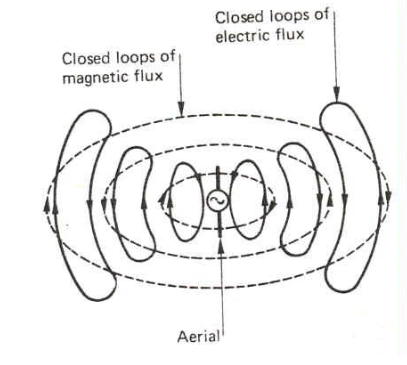
\includegraphics[width=0.35\textwidth]{img/champAntenne.png}
		\end{figure}
		
		\textbf{Onde TEM} (Transverse Electrique-Magnétique), c'est un mode de propagation tel que les champs électrique et magnétique sont tous les 2 orthogonaux a la direction de propagations.
		\begin{figure}[htp]
			\centering
			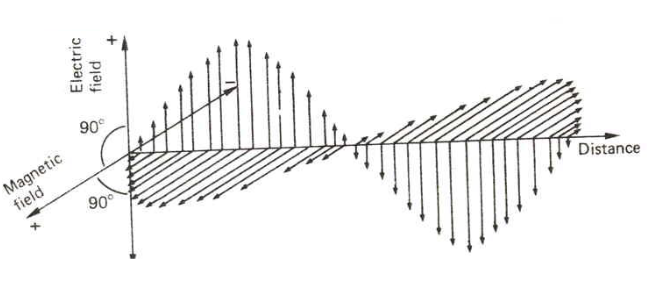
\includegraphics[width=0.45\textwidth]{img/TEM.png}
		\end{figure}
		
		\textbf{Rayonnement} : Quand l'antenne envois une rayonnement dans une direction, elle provoque aussi un rayonnement inverse non désiré. Ce rayonnement a un angle d'ouverture de $\omega$. On peut en mesurer le gains : 
		\begin{equation}
			\text{Gain} = \cfrac{\text{puisasnce dans la direction de puissance max}}{\text{Puissance dans cette direction si l'antenne etais isotrope}}
		\end{equation}
		
		\begin{minipage}{.5\textwidth}
  \centering
  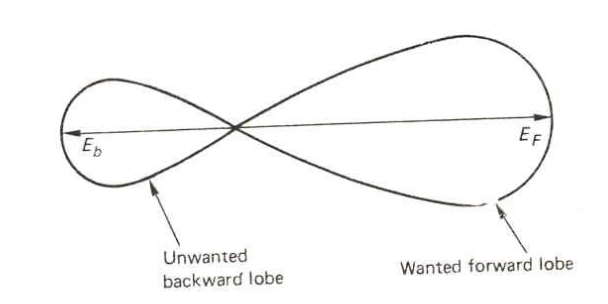
\includegraphics[width=.6\textwidth]{img/rayonnement.png}
\end{minipage}%
\begin{minipage}{.5\textwidth}
  \centering
  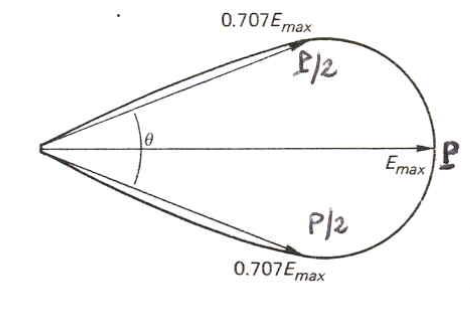
\includegraphics[width=.6\textwidth]{img/rayonnement2.png}
\end{minipage}
\begin{minipage}{.5\textwidth}
  \centering
\end{minipage}

	Il arrive que les ondes envoyé par des antennes, rencontre des objets/obstacle (couche inosphérique, batiment...). Ces objets reflete les ondes et entraine un problème de trajet multiple. C'est un problème qui fait que le meme signal arrive a des moments différents chez le récepteur ce qui entraine des dispersion et de la désynchronisation du signal. On sait que un signal qui varie vite a plus de chance d'avoir un problème de trajet multiple
	
	Il existe différent type d'antennes :
	
	\subsubsection{Dipole $\lambda/2$}
	
		\begin{figure}[htp]
			\centering
			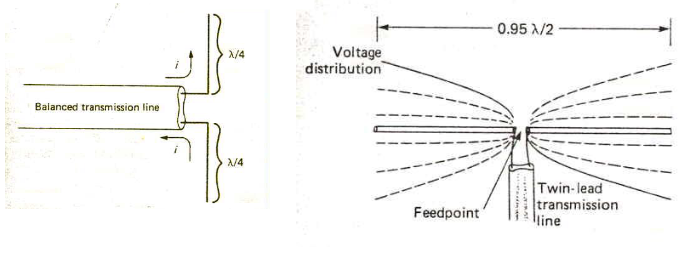
\includegraphics[width=0.7\textwidth]{img/dipole.png}
		\end{figure}
		
		c'est une antenne avec 2 tige de taille $\lambda /4$, les tension au centre sont minime et maximales en extrémité
	
		\begin{minipage}{.6\textwidth}
  \centering
  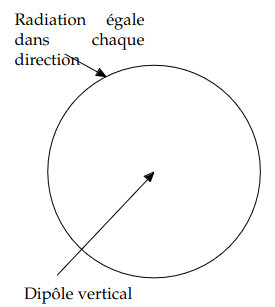
\includegraphics[width=.5\textwidth]{img/dipole1.png}

\end{minipage}%
\begin{minipage}{.5\textwidth}
  \centering
  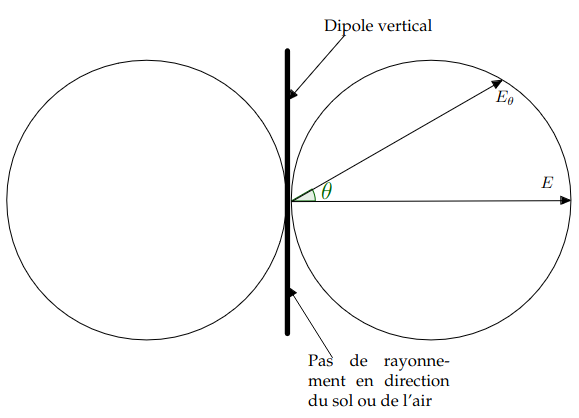
\includegraphics[width=.8\textwidth]{img/dipole2.png}

\end{minipage}
\begin{minipage}{.5\textwidth}
  \centering
\end{minipage}
		On peut minimiser l'antenne avec le principe de miroir qui reflète et simule le signal de l'autre branche.
		
	\subsubsection{Endfire}
		2 dipole de longueur $\lambda/2$ séparé par $\lambda/4$, l'antenne de droite alimente avec une avance de phase de 90° (donc $\lambda/4$) se qui entraine en renforcement vers la gauche
		
		\begin{figure}[htp]
			\centering
			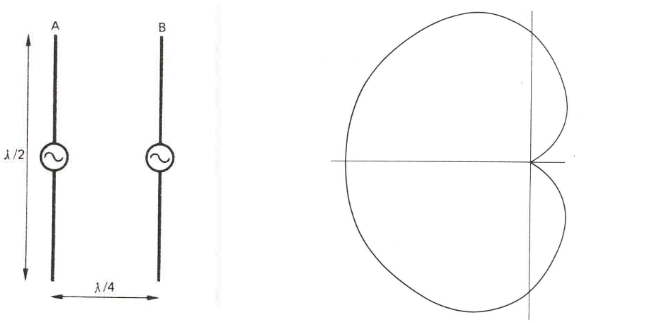
\includegraphics[width=0.6\textwidth]{img/endfire.png}
		\end{figure}
		
	\subsubsection{Yagi}
		Meme principe que les antennes endfire. Composé d'un réflecteur, dipôle et d'un directeur. Antennes très précise car directivité tres étroite. On peut augmenté la directivité en ajoutant des directeur mais diminue la bande passante
		
		\begin{figure}[htp]
			\centering
			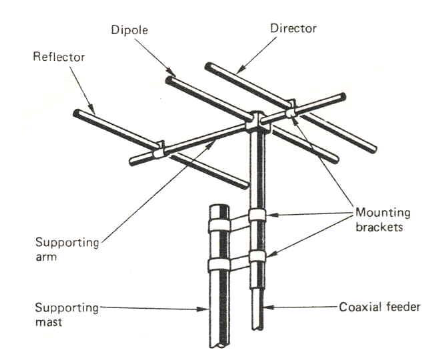
\includegraphics[width=0.35\textwidth]{img/yagi.png}
			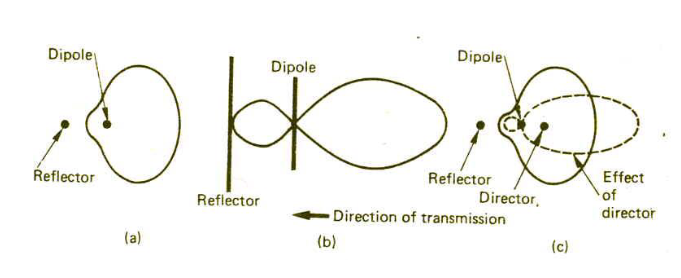
\includegraphics[width=0.55\textwidth]{img/yagi2.png}
		\end{figure}
		
	\subsubsection{Parabolique}
	
		Utilise une parabole pour émettre/recevoir un signal en le point centre de la parabole
		
		\begin{figure}[htp]
			\centering
			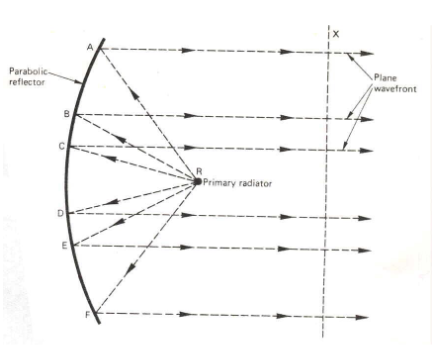
\includegraphics[width=0.45\textwidth]{img/parabole.png}
			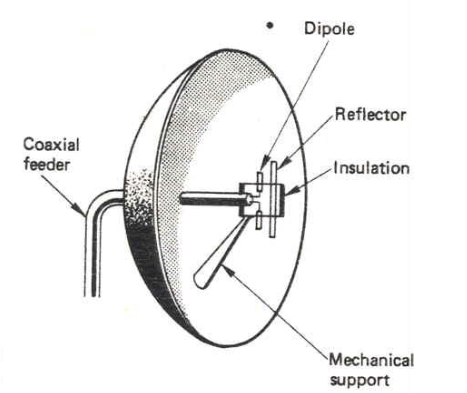
\includegraphics[width=0.45\textwidth]{img/parabole2.png}
		\end{figure}
	\subsubsection{Réseau d'antenne}
		Utilisé pour récuperer un signal faible en "agrégant" des signaux similaire
		\begin{figure}[htp]
			\centering
			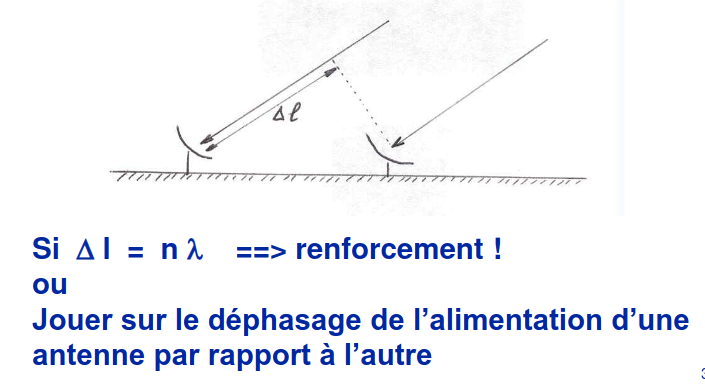
\includegraphics[width=0.7\textwidth]{img/reseauAntennes.png}
		\end{figure}


\newpage		

\section{Modulation}
	On va voire comment greffer l'information sur un signal.
	
	La \textbf{modulation} permet de transposer un signal (signal modulant) autour d'une autré fréquence (fréquence porteuse). Le signal modulé ressemble a une sinusoide et la variation contient l'information du signal modulant:
	\begin{equation}
		v_x(t) = A_c \cos(w_ct + \varphi_c)
	\end{equation}
	Il y a 3 type de modulation:
	\begin{itemize}
		\item modulation d'amplitude (joue sur $A_c$)
		\item modulation de fréquence (joue sur $w$)
		\item modulation de phase (joue sur $\varphi_c$)
	\end{itemize}
	
	dans cette section nous allons voire la modulation analogique
	
	\subsection{Modulation en bande de base}
		Bon j'ai m'enti il y en a 4.
		La transmition est dite en bande de base si elle ne subit aucune transposition de fréquence par modulation. Les fréquences initials du signal émis sont donc préservé.
	\subsection{Modulation d'amplitude (AM)}
		
		\begin{figure}[htp]
			\centering
			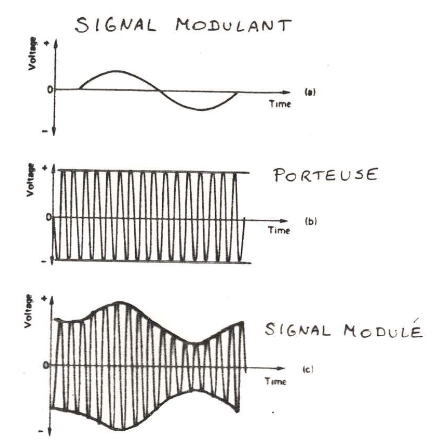
\includegraphics[width=0.4\textwidth]{img/modulationAM.png}
		\end{figure}
		
		Avec une porteuse et un signal modulant, on crée le signal modulé en appliquant les changements d'amplitude du signal modulant. Avec $s(t)$ le signal et l'on sait que $\varphi_c = 0$ on a :
		\begin{equation} \label{eq1}
			\begin{split}
		v_x(t) &= A_c \cos(w_ct + \varphi_c) \\
		v_{AM}(t) &= A_c \cos(w_ct) + ms(t) A_c \cos(w_c t) \\
		& = A_c[1+ms(t)]\cos(w_c t)
			\end{split}
		\end{equation}
		
		L'amplitude est multiplié par $(1+ms(t))$. Si $m$ (indice de modulation) est trop grand on a une \textbf{surmodulation} et donc une perte de l'information
		\begin{figure}[htp]
			\centering
			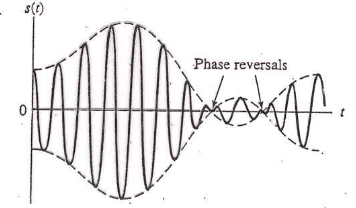
\includegraphics[width=0.4\textwidth]{img/surmodulation.png}
		\end{figure}
		
		\subsubsection{Modulation autour d'un porteuse}
			Rappel de Fourier:
			\begin{equation} \label{eq1}
			\begin{split}
				f(t) &\Leftrightarrow F(\omega)\\
				f(t-t_0) & \Leftrightarrow F(\omega) \exp(-jwt_0)\\
				f(t) \exp(jt\omega_0) &\Leftrightarrow F(\omega - \omega_0)\\
				f(t) \exp(-jt\omega_0) &\Leftrightarrow F(\omega + \omega_0)\\
				f(t) \cos(\omega_0 t) &\Leftrightarrow \cfrac{F(\omega + \omega_0) + F(\omega - \omega_0)}{2}
			\end{split}
		\end{equation}
		
		\begin{figure}[htp]
			\centering
			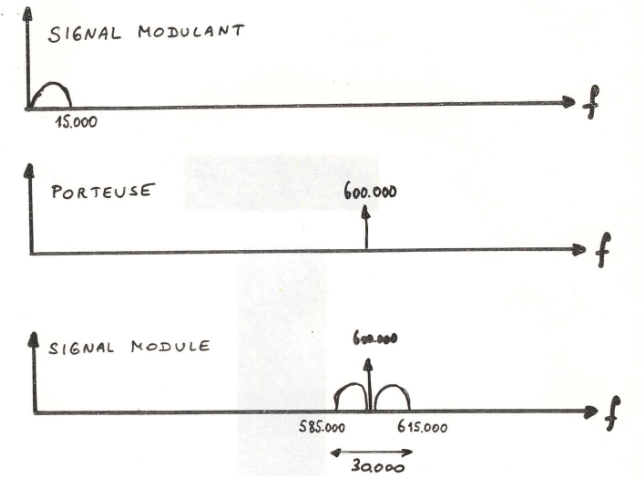
\includegraphics[width=0.4\textwidth]{img/modulationAM1.png}
			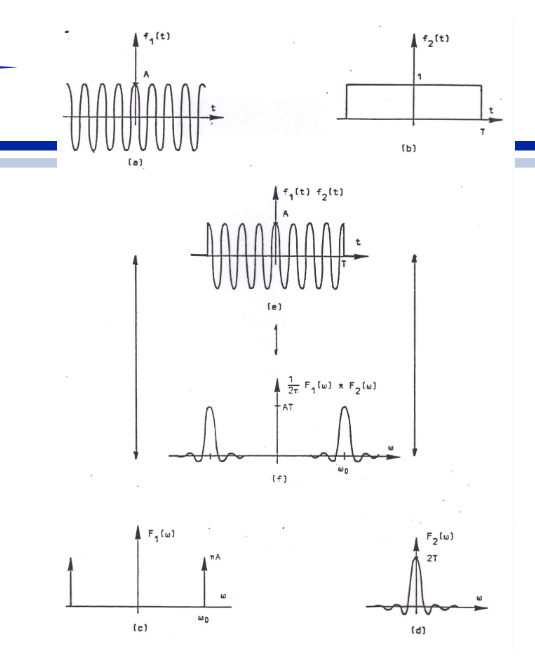
\includegraphics[width=0.4\textwidth]{img/modulationAM2.png}

		\end{figure}
			
		Multiplier le signal par la porteuse $\cos(\omega_0 t)$ en terme de Fourier, consiste de décaler le spectre des fréquences de $\omega_0$ dans les 2 sens autour de la porteuse. Il y aura donc des fréquences "\textit{négative}"
			
		\begin{figure}[htp]
			\centering
			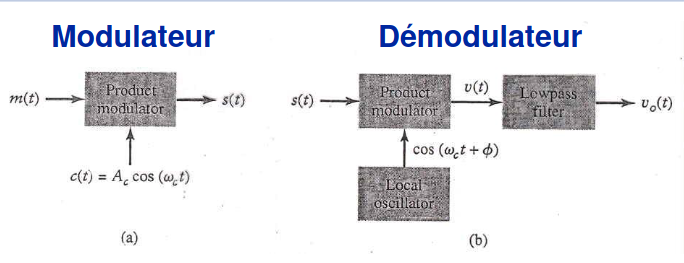
\includegraphics[width=0.6\textwidth]{img/modulationAM3.png}
		\end{figure}
		
		\textbf{Modulation :} le signal modulant $m(t)$ multiplié par une cosinusoïde résulte par le signal modulé $s(t)$
	
		\textbf{Démodulation :} le signal modulé $s(t)$ multopilié par la meme cosinusoïde que pour la modulation resulte en $v(t)$ et permet de retrouver le signal d'origine autour de la fréquence 0 sur la lequel on vient d'appliquer un filtre passe-bas pour conserver que le signal qui nous interesse.
			
			
		Le signal sortant du démodulateur ressemble a :
		
		\begin{equation} \label{eq1}
			\begin{split}
				p(t) &= A_c s(t) cos (\omega_c t + \varphi_c).\cos(\omega_c t + \varphi_c)\\
				&= A_c s(t) cos^2 (\omega_c t + \varphi_c).\cos(\omega_c t + \varphi_c)\\
				&= A_c s(t) \cfrac{A + cos(2\omega_c t + 2\varphi_c)}{2}
			\end{split}
		\end{equation}
		
		On va filtrer en passe-bas pour retrouver $s(t)$
		
		\subsubsection{Filtrage}
			Permet de filtrer un signal résultant d'un modulateur pour garder les composant interessant du contenu fréquentiel
			
			\begin{figure}[htp]
			\centering
			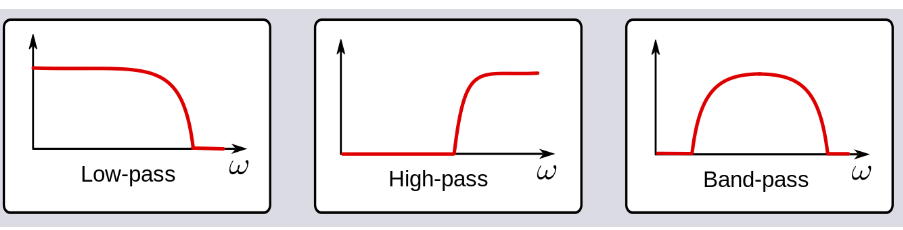
\includegraphics[width=0.6\textwidth]{img/filtrage.png}
			\end{figure}
			
			la fréquence de coupure $(freq_{coup})$
			
			\begin{itemize}
				\item \textbf{Filtre passe-bas (low-pass)} : Garde les composantes du contenu fréquentiel \textbf{en dessous} de la $freq_{coup}$ et retire celle \textbf{au dessus}
				\item \textbf{Filtre passe-haut (High-pass)} : Garde les composant du contenu fréquentiel \textbf{au dessus} et retirer celle \textbf{en dessous}
				\item \textbf{Filtre passe-bande (Band-pass)} : Garde les composantes du contenu fréquentiel \textbf{entre} la $freq_{coup\_1}$ et la $freq_{coup\_2}$ (ou $freq_{coup\_1} < freq_{coup\_2}$) et retire le reste.
			\end{itemize}
		
		\subsubsection{Bandes latérales}
			Comme dit précédemment, de fréquence "négatives" sont envoyé il est donc inutile d'envoyé 2 fois la meme info. Envoyé 2 bande latéral est suffisant que on reconstruit apres. Il y a 2 moyen pour savoir quelle bande envoyé.
			\begin{itemize}
				\item USB (upper side band) envoi les deux aux extrémité
				\item LSB (Lower side band) envoi les 2 au centre
			\end{itemize}
			
						
			\begin{figure}[htp]
			\centering
			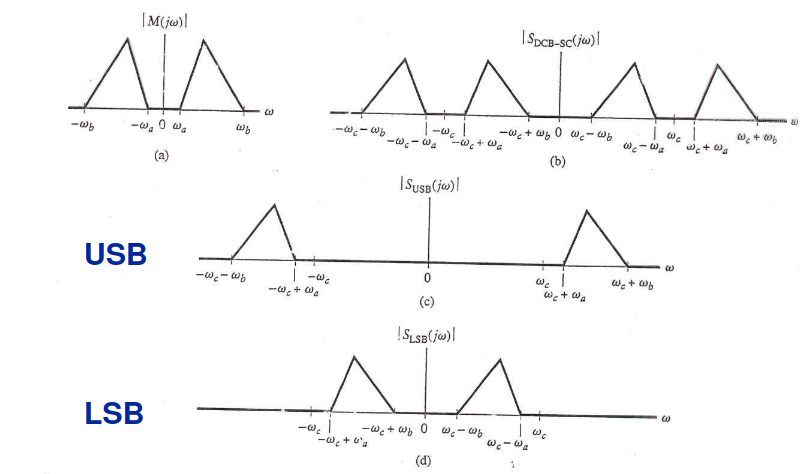
\includegraphics[width=0.6\textwidth]{img/BandeLateralUnique.png}
		\end{figure}
		
	\subsection{A CONTINUER}

\newpage

\section{Application}
	\subsection{Réception superhétérodyne}
		un réception superhétérodyne est un récepteur conçu sur le principe de mélange de fréquences. Permet de convertir le signal reçu en une fréquence intermédiaire plus basse qui est plus facile a utiliser. Avec une fréquence plus faible, ils est plus facile d'amplifier et de démoduler.
	
		\begin{equation}
			 f_{IF} = f_{rx}-f_{local}
		\end{equation}
		\begin{equation}
			 f_{IF} = f_{local}-f_{rx}
		\end{equation}
		
		les 2 fréquence sont symétriques autour de $f_{local}$ et on récupère (13) qui est la fréquence plus basse du signal recu via un filtre passe-bas
		
	\subsection{Radio}
		\subsubsection{Pouquoi plus radio FM que AM ?}
			\begin{itemize}
				\item \textbf{AM :} entre 600 et 900 kHz donc = 300kHz donc $\cfrac{300kHz}{30kHz} \approx 10$ donc asser de place pour 10 chaines de radio
				\item \textbf{FM :} entre 85 et 105 MHz donc 23MHz donc $\cfrac{23 000 MHz}{30kHz} \approx 766$ donc asser de place pour 766 chaines de radio
			\end{itemize}
			
		\subsection{Signal stéréo Radio}
			C'est la composition de plusieurs signaux formant un signal composite :
			\begin{itemize}
				\item G+D signal mono
				\item G-D signal supplémentaire pour crée le stéréo
			\end{itemize}
		
			\subsubsection{Modulation}
				
				Création du signal composite dans une bande FM:
				
				Un signal mono (G+D) + un modulation AM contenant a la fois G+D et G-D + pilote = porteuse de 30kHZ divisé par 2 sinon interférence avec le signal G-D
				
				\begin{figure}[htp]
				\centering
				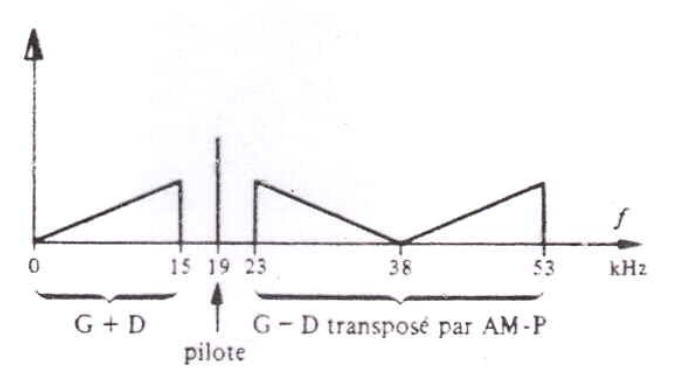
\includegraphics[width=0.6\textwidth]{img/signalStéréo.png}
				\end{figure}
			
			\subsubsection{Emetteur}
				Permet la création du signal stéréo
				
				\begin{enumerate}
					\item on a 2 signaux $x_L$ et $x_R$ pour gauche et droite
					\item on va former $x_L + x_R$ (G+D) et $x_L - x_R$
					\item on crée un sinusoîde localement a 38 kHz
					\item on la multiplie avec $x_L - x_R$ pour former G-D transposé comme sur la figure au dessus
					\item on divise par 2 la fréquence de la sinusoïde pour crée le pilote de 19 kHz
					\item on additione $x_L + x_R$, $x_L - x_R$ et le pilote et la somme vont former le signal composite qui est envoyé par le modulateur
				\end{enumerate}
				
				\begin{figure}[htp]
				\centering
				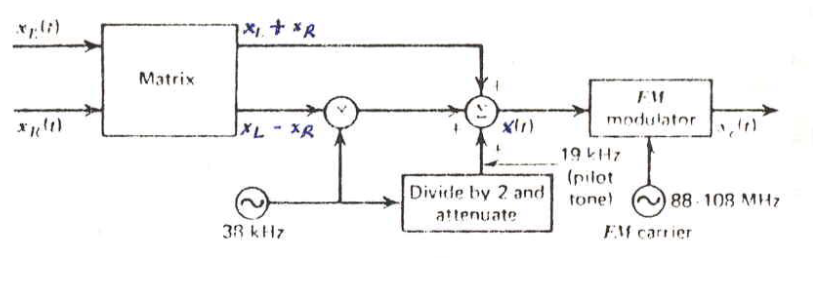
\includegraphics[width=0.6\textwidth]{img/emeteurStereo.png}
				\end{figure}
				
			\subsubsection{Récepteur stéréo }
				
				Permet la réception du signal mono ou stéréo
				
				\begin{enumerate}
					\item Effectue une démodulation FM pour récupéré le signal composite
					\item récupere G+D\\
						(a) utilise un filtre passe-bas 15 kHz (c'est la seul donnée nécessaire pour le MONO)
						
					\item recupere le pilote\\
						(a) utilise un filtre passe-bande 19kHz\\
						(b) multiplication de la fréquence du pilote par 2  pour crée porteuse de 38 kHz
					\item récupère G-D transposé \\
						(a) utilise un filtre passe-bande entre 23kHz et 53kHz
					\item démodulation du signal G-D transposé avec la porteuse de 38kHz (centre le signal autour de 0)
					\item utilise un filtre passe-bas de 15 kHz pour récuperer le signal original G-D
					\item Recombinaison des signaux G-D G+D pour crée le signal stéréo
				\end{enumerate}
				
				\begin{figure}[htp]
				\centering
				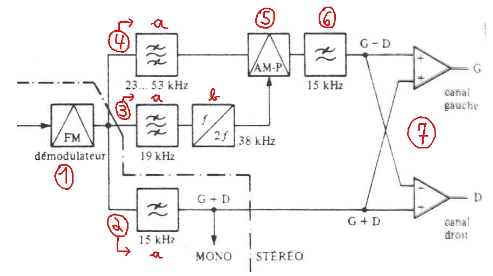
\includegraphics[width=0.6\textwidth]{img/recepteurStereo.png}
				\end{figure}
		\subsection{TV noir et blanc}
			\subsubsection{Modulation}
				 Création d'un signal composite contenant
				 \begin{itemize}
				 	\item signal vidéo (porteuse a $\approx$ 4 MHz)
				 	\item signal audio (porteuse a $\approx$ 4.5 MHZ) modulé en FM
				 	
				 \end{itemize}
				 
				 \begin{figure}[htp]
				\centering
				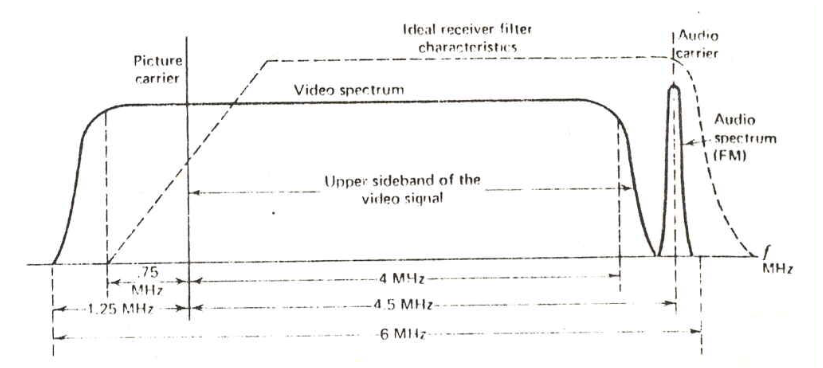
\includegraphics[width=0.7\textwidth]{img/ModulationTVNoirBlanc.png}
				\end{figure}
			\subsubsection{Emetteur}
				\textbf{Audio} : 
				\begin{enumerate}
					\item Recupere le signal audio grace au micro
					\item utilise le modulateur de fréquence audio 4.5 MHz (audio carrier) pour faire une modulation FM du signal audio\\
					
				\textbf{Vidéo} : \\
					\item Récupere signal audio par la caméra
					\item Utilise modulateur de fréquence vidéo (vidéo carrier) pour faire modulation AM du signal vidéo\\
					
				\textbf{Final} :\\
				
				\item additionner signal audio et vidéo
				\item modulation du resultat des signaux (VSB filter)
				\end{enumerate}
				
				\begin{figure}[htp]
				\centering
				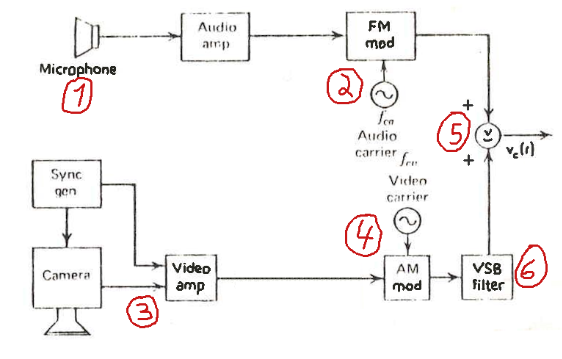
\includegraphics[width=0.7\textwidth]{img/EmetteruTVNoirBlanc.png}
				\end{figure}
				
			\subsubsection{Recepteur}
				Permet réception signal TV noir et blanc
				\begin{enumerate}
					\item récupération signal par antenne
					\item Démodulation pour arriver a une fréquence intermédiaire
					\item Démodulation FM pour récupérer signal audio
					\item Démodulation AM pour récupérer signal vidéo
					
				\end{enumerate}
				
				\begin{figure}[htp]
				\centering
				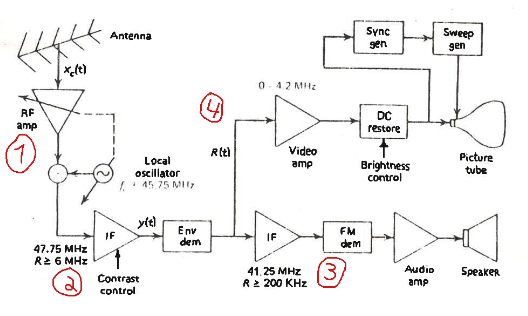
\includegraphics[width=0.7\textwidth]{img/recepteurTVNoirBlanc.png}
				\end{figure}
		\newpage
		\subsection{TV couleurs}
			\textcolor{red}{R} \textcolor{green}{G} \textcolor{blue}{B} $\Rightarrow$ Y U V
			
			Y = 0.30 \textcolor{red}{R} + 0.59 \textcolor{green}{G} + 0.11\textcolor{blue}{B}
			
			U = 0.493 (\textcolor{blue}{B} - Y)
			V = 0.877 (\textcolor{red}{R} - Y)
			
			Y = luminance $\Rightarrow$ signal de noir et blanc
			U et V = Chrominances $\Rightarrow$ Signaux pour récupéré les info de couleurs
			
			On envois 3 signaux de couleur R G B pour pouvoir continuer a utilise les tv en noir et blanc (Y)
			
			\subsubsection{Système NTSC}
				Luminance : VSB
				
				Chrominances : QAM
				
				Son : FM
				
				\begin{figure}[htp]
				\centering
				\includegraphics[width=0.6\textwidth]{img/NTSC.png}
				\end{figure}
			\subsubsection{Système PAL}
				Facilite la démodulation QAM des chrominances
				\begin{equation}
					v(t) = U\sin (\omega_c t) \theta \pm V \cos (\omega_c t)
				\end{equation}
				
				Le $\pm$ fait tous, $\Rightarrow$ "Phase alternating line" : Plus de tolérance pour les erreurs de phase
				
				\begin{itemize}
					\item U et V avec la meme largueur de bande
					\item Spectre (contenue fréquentiel) plus compliqué
					\item Porteuse plus éloignée
				\end{itemize}
				
				\begin{figure}[htp]
				\centering
				\includegraphics[width=0.7\textwidth]{img/PAL.png}
				\end{figure}
				
			\subsubsection{Création du signal PAL}
			
			\begin{figure}[htp]
				\centering
				\includegraphics[width=0.7\textwidth]{img/PAL1.png}
			\end{figure}
				
				
			\subsubsection{Systheme SECAM}
				"Séquentiel a mémoire"
				
				On ne transmet chaque chrominance qu'une ligne sur 2 et on les moduel en FM pour eviter les difficulté de la QAM
				
		\subsection{TV numérique}
			y = 0.299 \textcolor{red}{r} + 0.587 \textcolor{green}{g} + 0.114 \textcolor{blue}{b}
			
			Y = 219 y + 16
			
			CR = $\cfrac{112(\textcolor{red}{r} - y)}{0.701} + 128$
			
			CB = $\cfrac{112(\textcolor{blue}{b} - y)}{0.886} + 128$
			
			
			La luminance : Y echantillonné a 13.5MHz (864 ech/ligne)
			13.5MHz car :
			\begin{itemize}
				\item Theoreme de Shannon ($f_{ech} > 2 f_{MAX}$)
				\item On travaille sur une bande de max 6MHz cf Systeme PAL
				\item Le signal vidéo a donc une fréquence de 6MHz
				\item La fréquene d'echantillionnage doit etre plus grande que 12MHZ ($f_{ech} > 12MHz$)
			\end{itemize}
			
			CR et CB (signaux de chrominance) sont echnatiollonées a 6.75 MHZ (432 ech/ligne)
			
			Quantification 8 bits/echantillions $\Rightarrow$ 216Mbs avant compression
			
			\textbf{Avantages}:
			\begin{itemize}
				\item compression
				\item Code correcteur erreurs + "regénérations"
				\item Qualité optimale dès que la transmission est assez bonne
				\item Permet de transmettre + de cannaux dans la même bande
				\item Possibilités d’enregistrements, etc \dots 
			\end{itemize}
			
			\textbf{Désavantages}
			\begin{itemize}
				\item Délais de zapping (codage)
				\item Dégradation rapide si mauvais signal
			\end{itemize}

\newpage

\section{Transmission de données}
\label{TDD}
	\subsection{Protocoles de liaison}
		Le protocole définit le format de la trame avec de bit de controles:
		\begin{itemize}
			\item Source/dest
			\item Etablissement de la liaison
			\item Gestion de l'acces
			\item \dots
		\end{itemize}
		
		Certains role important :
		\begin{itemize}
			\item Medium acces control (MAC)
			\begin{itemize}
				\item Gere le multiplexage entre utilisateur du lien PHY
				\item centralisé ou distribué
				\item ex : 4G/GSM/LTE/\dots
			\end{itemize}
			\item Firward Error Correction (FEC)
			\begin{itemize}
				\item Codes correcteurs d'erreurs
			\end{itemize}
			\item Automatic Repeat Request  (ARQ)
			\begin{itemize}
				\item Mécanisme de retransmition 
			\end{itemize}
		\end{itemize}
		
	\subsection{MAC : Multiplexage}
		\subsubsection{Frequency Domain Multiple Access (FDMA)}

			Principe des différentes radio FM : Chaque radio a une place en fréquence attribuée, Utilisé pour répartir plusieur utilisateurs dans un systeme
			\begin{figure}[htp]
				\centering
				\includegraphics[width=0.7\textwidth]{img/FDMA.png}
			\end{figure}
		
		\subsubsection{Time Domain Multiple Access (TDMA)}
			Meme principe que FDMA
			
			Definitions d'une période de temps qui va se répéter et  qui est diviése en timeslots TDMA. Un timeslot est attribuée a un utilisateur et ne poura envoyer que pendant le timeslot asssigné a chaque période répétitives.
			
			\begin{figure}[htp]
				\centering
				\includegraphics[width=0.7\textwidth]{img/TDMA.png}
				\includegraphics[width=0.7\textwidth]{img/TDMA1.png}
			\end{figure}
		\subsubsection{Code Division Multiple Access (CDMA)}
		
			Pour diviser les utilisateurs  on utilise plus le temps ou la fréquence mais un code (comme pour le 3G)
			
			Contient 3 signaux:
			\begin{itemize}
				\item \textbf{Data Signal :} Signal binaire composé d'une période $T_b$ (durée d'un bit d'info envoyé)
				\item \textbf{PseudoRandom Code :} Code spécifique à chaque utilisateur permettant d'encoder/moduler le data signal
				
				La durée du \textit{Chip} ($T_c < T_b$)
				\item \textbf{Transmitted signal} : Signal transmit qui est le resultat d'un application XOR avec le \textbf{Data signal} et \textit{PseudoRandom Code}
			\end{itemize}
			
			\begin{figure}[htp]
				\centering
				\includegraphics[width=0.7\textwidth]{img/CDMA.png}
			\end{figure}
			
	\subsection{Gestion des erreurs}
		\subsubsection{Causes des erreurs}
			\begin{itemize}
				\item Dispersion dans les lignes
				\item Bruit thermique
				\item Bruit Impulsif
				\item Echos/diaphonie
				\item Perte de synchro
				\item Effet "amplifiés" en fonction de l'atténuations
			\end{itemize}
			
		\subsubsection{Code détecteur et correcteur d'erreur}
		
			Principe de base : envoyer de le redondance
			
			\textbf{Ex1:} Code de parité :
				
				Verifier si le nombre de bits est paire ou impaire pour chaque période d'envois
				
				Limité si on on a des erreurs doubles dans le meme bloc
				
				\begin{figure}[htp]
					\centering
					\includegraphics[width=0.3\textwidth]{img/Erreur.png}
				\end{figure}
				
			\newpage
				
			\textbf{Ex2 :} Langues/dictionnaire de mots valables
			
			\begin{figure}[htp]
				\centering
				\includegraphics[width=0.7\textwidth]{img/Erreur2.png}
			\end{figure}
			
			\textbf{Ex3 : }Code a répétition
		
				Répété chaque bit envoyé 1 fois :
				\begin{itemize}
					\item 0 $\rightarrow$ 00
					\item 1 $\rightarrow$ 11
				\end{itemize}
				
				donc 00 et 11 sont correcter et 01 et 10 sont faux
				
			\textbf{Ex4 : }Code a double répétition
				Répété chaque bit envoyé 2 fois :
				\begin{itemize}
					\item 0 $\rightarrow$ 000
					\item 1 $\rightarrow$ 111
				\end{itemize}
				
				donc 000 et 111 sont correcte et 001, 010, 011, 100,101 et 110 sont faux
				
			\textbf{Ex5 :} Code de Hamming
				Code(15,11)
				
				i = 1 0 1 0 1 0 1 1 0 0 1
				
				On a :
				\begin{itemize}
					\item 11 bits entrée
					\item 15 bits codé $\rightarrow$ 4 bits de redondance/parité
				\end{itemize}
				
				On place les bits de codage au rangs de "puissance de 2" pour déterminer les 4 bits de rédondance
				
				\begin{tabular}{ccccccccccccccc}
					15 & 14 & 13 & 12 & 11 & 10 & 09 & 08 & 07 & 06 & 05 & 04 & 03 & 02 & 01\\
					1 & 0 & 1 & 0 & 1 & 0 & 1 & $c_4$ & 1 & 0 & 0 & $c_3$ & 1 & $c_2$ & $c_1$ 
				\end{tabular}
				
				Ensuite on prend les rangs avec un bit = 1
				
				\begin{tabular}{c|c}
				15 & 1 1 1 1\\\hline
				13 & 1 1 0 1\\\hline
				11 & 1 0 1 1\\\hline
				9  & 1 0 0 1\\\hline
				7  & 0 1 1 1\\\hline
				3  & 0 0 1 1
				
				\end{tabular}
				
				Ensuite on calcule le module 2 (en additionnant les valeurs de chaque colones d'avant avec 0 si paire et 1 si impaire)
				
				\begin{tabular}{cccc}
				1 & 1 & 1 & 1\\
				1 & 1 & 0 & 1\\
				1 & 0 & 1 & 1\\
				1 & 0 & 0 & 1\\
				0 & 1 & 1 & 1\\
				0 & 0 & 1 & 1\\ \hline
				0 & 1 & 0 & 0\\
				$c_4$ & $c_3$ & $c_2$ & $c_1$
				
				\end{tabular}
				
				On peut verifier  car seulement $c_3$ contient un 1 et est a la position 4 (0100)
				
				\begin{tabular}{cccc}
				1 & 1 & 1 & 1\\
				1 & 1 & 0 & 1\\
				1 & 0 & 1 & 1\\
				1 & 0 & 0 & 1\\
				0 & 1 & 1 & 1\\
				0 & 0 & 1 & 1\\ 
				\textcolor{green}{0} & \textcolor{green}{1} & \textcolor{green}{0} & \textcolor{green}{0}\\\hline
				\textcolor{red}{0} & \textcolor{red}{0} & \textcolor{red}{0} & \textcolor{red}{0}\\
				$c_4$ & $c_3$ & $c_2$ & $c_1$
				
				\end{tabular}
				
				Réception d'un message avec une erreur :
				
				\begin{tabular}{ccccccccccccccc}
					15 & 14 & 13 & 12 & 11 & 10 & 09 & 08 & 07 & 06 & 05 & 04 & 03 & 02 & 01\\
					1 & 0 & 1 & 0 & 1 & 0 & \textcolor{red}{0} & 0 & 1 & 0 & 0 & 0 & 1 & 0 & 0 
				\end{tabular}
				
				Et donc on fait comme avant et on calcule le modulo 2
				
				\begin{tabular}{cccc}
				1 & 1 & 1 & 1\\
				1 & 1 & 0 & 1\\
				1 & 0 & 1 & 1\\
				0 & 1 & 1 & 1\\
				0 & 1 & 0 & 0\\
				0 & 0 & 1 & 1\\ \hline
				\textcolor{red}{1} & \textcolor{red}{0} & \textcolor{red}{0} & \textcolor{red}{1}
				
				\end{tabular}
				
				Et donc \textcolor{red}{1} \textcolor{red}{0} \textcolor{red}{0} \textcolor{red}{1} = 9 donc le bit 9 est érroné
				
			\textbf{Avantage} :
			\begin{itemize}
				\item redondance minimale pour la capacité correctrie voulue a la taille du bloc voulue
				\item facile a réaliser
				\item Peut trouver une seule erreur dans le block (inconvénient)
			\end{itemize}
			
		\subsubsection{Codes et redondance}
			ajouter de la redondance = certains mots sont correct et d'autre incorrect
			
			Cela permet détection/correction. Si on a plus de redondance, on a plus de mots espacés et donc avoire de meilleur possibilités de detections/corrections et mais cela a un cout en débit a transmettre
			
		\subsubsection{Code VS. encodage}
			En fonction du code/dictionnaire ça va impacté sur les performances
			
			Choix de l'encodage  = Table d'entrée / sortie du codeur
			
			\begin{tabular}{|c|c|}
			\hline
			Input & Output\\ \hline
			000 & 000000 \\ \hline
			001 & 001111 \\ \hline
			010 & 010100 \\ \hline
			011 & 011101 \\ \hline
			\dots & \dots \\ \hline
			
			\end{tabular}
			
			Avec $k$ bits d'entrée et $n$ bit de sortie, on peut déterminer que :
			\begin{equation}
				\# \text{mots code} = n = 2^k
			\end{equation}
			
		\subsubsection{Théorie des codes}
		
			Comment ajouter de la redondance/définir le dictionnaire pour obtenir de bonnes capacité correctrices/détectrices en augmentant le débit de moins possible
			
			Distance de Hamming:
			
			Code($n,k$) Soit $k$ le nombre de bits utile et $n$ tel que $n-k$ est le nombre de bits de controle. Le \textbf{Taux du code} est $k/n$. On va choisir dans le dico le mots le plus proche trouvé en utilisant la distance. \textbf{code(n,k)} est de distance minimal $d$ détecte les erreurs d'ordre d-1 et corriges les erreurs d'ordre $\textit{floor[(d-1)/2]}$
			
			ex : 
			\begin{tabular}{c}
			0001101\\
			\textcolor{red}{1}001\textcolor{red}{0}01
			\end{tabular}Distance de 2
			
			ex2:
			
			\begin{tabular}{c}
			000OO\\
			11111
			\end{tabular} on a reçu 11010, d(00000,11010) = 3 et d(11111,11010) = 2 on choisis donc 11111
			
			
			TODO:A terminer
		
\newpage
		
\section{Compression}
	But : Reduire la taille de objets pour économiser de l'espace sans pour autant détruire les fichiers. Ex : 50 films de 1min en 480p = 82GB ($640 \times 480 \times 24 \times \times 30fps = 27MB/film$).

	Les données peuveut etre comprimé a environs :
	\begin{itemize}
		\item text 2:1
		\item image 5:1
		\item son stéréo 6:1
		\item Vidéo 50:1
	\end{itemize}
	
	2 grande familles de compression:
	\begin{itemize}
		\item Sans perte (lossless)
		\item Avec perte (lossy)
	\end{itemize}

	2 grand principes dans la compression, \textbf{supprimé redondance} et garder les caractéristique importante
	
	\subsection{Codage sans pertes}
		\subsubsection{Codage entropique}
			On utilise des codes court pour les mots redondants. Se base sur le concept d'entropie. \textbf{Entropie :} Limite théorique de l'information que l'on peut transmettre sur une canal
			
		\subsubsection{Code de Huffman}
			On construit un nouvel alphabet sur un arbre qui représente la probabilité de voir cette lettre. Arbre organisé tel que la branche de gauche est 0 et droite de 1. On commence au top et on met la lettre la plus problable a gauche, et le reste a droite, et on fait pareil a chaque niveau
			
			\begin{figure}[H]
				\centering
				\includegraphics[width=.5\textwidth]{img/Compression/Huffman.png}
			\end{figure}
			
		\subsubsection{Lempel-Ziv}
			Utilisé dans \textit{gzip}. On regarde les données que on a déja envoyé avant et on trouve le bout déja envoyé, on va spécifier a quelle distance il se situe du point actuel sur quelle longueur il s'etend.

			\begin{figure}[H]
				\centering
				\includegraphics[width=.5\textwidth]{img/Compression/L77.png}
			\end{figure}
			
	\subsection{Codage avec pertes}
		On va mesurer une \textit{distorsion} (somme des carres des erreurs ou Distance de hamming) qui va dire le taux d'erreur acceptable. Plus il est élevé, moin on a besion de débit pour les données
		
		\subsubsection{JPEG}
			Les block de 8x8 pixel de l'image sont remplacé par des matices de coefficients DTC de taille 8x8. Le but est de perdre que une parties des blocs de DCT. Virer des pixels non mais oublier un DCT ok
			
			On applique ensuite la \textbf{quantification} sur la matrice de coefficient DCT. On divise la matrice de pixel en matrice de quantification dans le but d'atténuer les hautes fréquences (presque insensible pour l'humain). Certains coefficient sont a 0 (en bas a droite de la matrice).
			
			Ensuite un codage en ZIG-ZAG permet de ne garder qu'un minimum de coéfficient et de se débarasser des nuls.
			
			\begin{figure}[H]
				\centering
				\includegraphics[width=\textwidth]{img/Compression/DCT.png}

			\end{figure}
			\begin{figure}[H]
				\centering
				\includegraphics[width=\textwidth]{img/Compression/DCT1.png}

			\end{figure}
			\begin{figure}[H]
				\centering
				\includegraphics[width=\textwidth]{img/Compression/DCT2.png}

			\end{figure}
			\begin{figure}[H]
				\centering
				\includegraphics[width=\textwidth]{img/Compression/DCT3.png}

			\end{figure}
	\subsection{Vidéo}
		Utilise le principe de prédiction (\textbf{Block matching algorithm}). Se base sur l'idée que 2 images successive d'un vidéo sont tres peu différente. Mais pendants changement de scene, il faut garder images au complet.
		
		Un peu comme JPEG mais avec une prédictions temporelle en plus
		
		3 types de frames :
		\begin{itemize}
			\item \textbf{Intraframe (I):} Image complete (1 à 2sec) 
			\item \textbf{Interfraime (P) :} Image prédite a partir d'une précédente
			\item \textbf{Bidirect (B) :} Prédite  a partie d'un précédente ou suivante. 
		\end{itemize}
		
		La prédiction consiste en la translation d'une série de block appartenant a l'image précédente utilisé
		
		Encodage complexe et lent mais décodage tres rapide
			Fixer niveau interférence admis	

\newpage

			
\section{Communications Mobiles}
	\subsection{GSM (2G)}
		Se base sur un systheme de cellules haxagonales de taille différente
		\begin{itemize}
			\item Macrocell (30km)
			\item Microcell (2-4km)
			\item Picocell (200m)
			\item Femtocell
		\end{itemize}
		
		Une tour associé a chaque cellules, les \textbf{BTS}(Base Transceiver Station). Ces tours sont associées en groupes a une station, les \textbf{BSC} (Base station controller). Enfin les BSC sont associé a un centre \textbf{MSC} (Mobile service switching center). Ces centre sont relié par 3G a internet.
		
		Les utilisateur communique avec les BTS.
		
	\subsection{Réutilisation des fréquences}
			On fixe un niveau admissible d'interférence entre les différents tours (elle utilise la meme fréquence), souvent a 10db. Il font donc réfléchir au placement des tours.
			\begin{figure}[H]
				\centering
				\includegraphics[width=0.7\textwidth]{img/CM/RF.png}
			\end{figure}
			
			On va utiliser un \textbf{Planning de fréquences}, qui va essayer de distribuer les fréquences entre les tours pour eviter au max les interférences.
 
 			\begin{figure}[H]
				\centering
				\includegraphics[width=0.5\textwidth]{img/CM/PF.png}
			\end{figure}
			
			Les bandes fréquences GSM \textbf{Montantes} (Envois donnée vers stations) est de 890 à 915 MHz et descendantes (Stations envoi donnée a user) 935 à 960 MHz
			
	\subsection{Modulations}
		GSM utilie \textbf{GMSK} (Gaussian minimum shift keying) pour l'envoi des données numérique la largueur de bande est de 200 kHz. Tres robuste mais peu efficace
		
	\subsection{Multiplexage}
 		Couplage du TDMA et du FDMA ( cf section Transmission des données)
 		
 		Chaque tour founit 8 timeslot et 124 cannaux de 200kHz. Deux utilisateurs peuvent partager un timeslots (\textbf{Half rate}, chacun son tour). Petit décalage entres les timesolts déscendant et montant.
 		
 		\begin{figure}[H]
 			\centering
 			\includegraphics[width=\textwidth]{img/CM/HR.png}
 		\end{figure}
 		
 		\subsubsection{Structure timeslot}
 			5 types de paquets (\textbf{burst}), l'emission d'un paquet  correspond a l'emission de 156.25 bits:
 			
 			\begin{itemize}
 				\item \textbf{Acces} : demande de contact avec le réseau
 				\item \textbf{Synchronisation} : Localisation + réception d'un fréquence pour communiquer
 				\item \textbf{Normal} : Envoi du message
 				\item \textbf{Correction fréquence} : Prévention d'interférence possible (burst vide)
 				\item \textbf{Bourrage} : Complete le vide
 			\end{itemize}
 			
 	\subsection{Distorsion}
 		Probleme est la perte du signal entre la tour et l'utilisateur, plusieur raisons
 		\begin{itemize}
 			\item \textbf{Multi-trajet} : Signal prends plusieur chemin pour rejoindre la station a cause des interférence (rebond sur un immeuble)
 			\item \textbf{Shadowing} : Un objet ostrue la transmission
 			\item \textbf{Effet doppler} Décalage de fréquence d’une onde entre l’émission et la réception quand la distance entre les deux varie au cours du temps. Cet effet est causé par le déplacement de l’utilisateur par rapport à l’antenne
 		\end{itemize}
 		
 		Plusieurs solutions :
 		\begin{itemize}
 			\item Codes correcteurs d'erreur
 			\item diversifier les fréquences du signal (Frequency hopping)
 			\item Jouer sur la modulation
 			\item Égalisation du signal
 		\end{itemize}
 		
 		\textbf{Frequency Hopping} : On transmet le premier burst a une fréquence $f_1$, la deuxieme a fréquence $f_2$ et le troisieme a $f_3$ et on réutilise ces fréquence dans cet ordre
 		
 		
 	\subsection{Alignement dynamique}
 		Si 2 utilisateurs utilise des timeslot différents maiq que leur distance a la tour varie, il est pas impossible que les signaux s'interfère.
 		
 		On doit adapter le time slot en fonction du temps que le signal va prendre pour arriver à la tour. Cela revient à ajouter du décalage temporel de façon à ce que la station de base tombe toujours bien sur le timeslot qu’il faut
 		
 		Ne peut se faire que en montant car il peut y avoir plusieur utilisateur. En descendant,  se serait ridicule puisqu’il n’y a qu’un seul destinataire possible. (le GSM ne parle qu’à la station alors que la station parle à beaucoup de GSM)
 		
 	\subsection{Accès au système}
 	
 		La premier connexion a la tour :GSM regarde les canaux libre et parle a la station qui va lui attribuer un canal et timeslots
 		
 		Arrive quand :
 		\begin{itemize}
 			\item premiere connexion
 			\item Pour initier un appel
 			\item Pour répondre a un appel
 			\item Envoyer ou recevoir des données
 		\end{itemize}
 		
 	\subsection{Handover}
 		Quand le GSM change de BTS en brisant l'ancienne et puis crée une nouvelle liaison. A lieu quand  un diminution de la qualitité et donc propose nouvelle BST au GSM (par MSC) 
 		
 	\subsection{Internet sur GSM}
 		\subsubsection{GPRS (2.5G)}
 			Utilise les paquet de transmission pour transmettre internet. On tranmet un paquet que quand necessaire car facturé au volume
 			
 			Debit de 40-100 kb/s
 			
 		\subsubsection{Edge (2.75G)}
 			Modualtion 8-PSK qui permet 3/4 fois plus de débit. Implique du matériél adapté sur les stations et terminaux.
 			
 		\subsubsection{UMTS (3G)}
 			Fréquence 1885-2025 MHz montant 2110-2200 MHz descendant. Compatible mondial. Largueur de bande de 5MHz
 			
 			On utilise W-CDM (Une sorte de CDMA)
 			\begin{itemize}
 				\item Plus d'alignement dynamique nécessaire
 				\item Soft handover possible
 				\item Plus d'interférence
 			\end{itemize}
 			
 			Vitesse :
 			\begin{itemize}
 				\item 2 Mb/s stations fixe (pietons)
 				\item 144 kb/s Sation mobile (en voiture)
 			\end{itemize}
 			
 		\subsubsection{LTE (4G)}
 			Utilise modulation OFDM (descendant) et SC-FDMA (montant). Tres flexible. Utilise des fréquences de 450Mhz a 3.8Ghz selon les pays et modulation adaptative qui permet d'adapter la constellation utilisé. Si la liaison est bonne alors on auraune constellation avec beaucoup de points permettant un meilleur debit. Si mauvaise liaison, constellation avec peut de points pour eviter les erreurs et donc debit plus faible.
 			
 			Différence avec anciens systheme
 			\begin{itemize}
 				\item \textbf{AMC} : \textit{Adaptative Modulation and Coding} : On adapte le débit à la qualité de la transmission. Si on a une transmission de qualité, on va augmenter la taille de la constellation pour augmenter le débit
 				\item \textbf{Multiplexage/modulation} : Modulation OFDM : Consiste à diviser le temps et les fréquences utilisables en un quadrillage où chaque carré représente une ressource. on va alors allouer aux utilisateurs des ressources de manière dynamique (adaptative) en fonction des besoins de l’utilisateur, du trafic, des interférences et/ou de la mobilité de l’utilisateur.
 				\item \textbf{Bande variable} : dû à l’OFDM, on peut utiliser une bande variante pour une transmission donnée. Cela rajoute une complexité au niveau des émetteurs et récepteurs 4G. 
 				\item \textbf{HARQ} : \textit{Hybrid Automatic Repeat reQuest} : Lorsqu’un bloc n’est pas acquitté, on ne retransmet pas toute la frame mais plutôt certains bits.
 			\end{itemize}

\newpage

\section{WIFI}
	Faire un réseau une seul cellule sur lequel les utilisateurs sont séparés en fréquences (FDMA). Bande wifi autour 2.4Ghz avec 14 bande 5Mhz avec un débit de 1 a 11MB/s
	\subsection{Modulation}
		Se fait en \textbf{DSSS}, aujourd’hui les nouveaux standards remplacent DSSS par OFDM. DSSS utilise du CDMA et possède une largeur de bande de 22Mhz, cette largeur couvre plusieurs canaux.
		
		Les nouveaux standards OFDM utilisent une sorte de FDMA. La bande est divisée en beaucoup de petites sous-bandes qui sont rendues indépendantes par le traitement du signal. Ce qui a un énorme impact sur la bande passante
		
		Le standard du futur est le MIMO (multiple input multiple output). Cette technique utilise plusieurs antennes en même temps. Ce standard lève 3 soucis de design :
		
		\begin{itemize}
			\item Beamforming : Le standard du futur est le MIMO (multiple input multiple output). Cette technique utilise plusieurs antennesen même temps. Ce standard lève 3 soucis de design :
			\item Multiplexage spatial : Les messages divisé doivent être réassemblé pour récuperer le canal sur lequel transite les données. 
			
				\begin{figure}[H]
					\centering
					\includegraphics[width=\textwidth]{img/wifi/M.png}
				\end{figure}
			\item Conbattre les évanouissement : La réception peut varier énormément d’un endroit à un autre. Comme il y a plusieurs antenne envoyant un signal il y a la possiblité qu’un signal arrive et l’on choisis le meilleur signal arrivant. Il faut évidemement que les antennes soit suffisement espacé (Au moins $\lambda$/2 ).
On lutte donc contre les trajets multiples !
		\end{itemize}
		
	\subsection{Standard}
		\begin{figure}[H]
			\centering
			\includegraphics[width=\textwidth]{img/wifi/S.png}
		\end{figure}
		

 			



\end{document}
